\documentclass[a4paper,11pt]{article}
\pdfoutput=1 % if your are submitting a pdflatex (i.e. if you have
             % images in pdf, png or jpg format)
\usepackage{upgreek,tipa,cancel,mathrsfs,mathtools,mdframed}
\usepackage{amssymb,amsfonts,amsmath, amscd, amsthm, amsfonts,bm,fontawesome,tcolorbox,xcolor}
\usepackage{jheppub} % for details on the use of the package, please
                     % see the JHEP-author-manual

\usepackage[T1]{fontenc} % if needed
	\def\gammma{		
		\text{\Large \textramshorns}
}
\newcommand{\dd}{\mathrm{d}}
\newcommand{\UHP}{\mathbb{H}}
\newcommand{\Hilbert}{\mathcal{H}}
\newcommand{\UD}{\mathbb{D}}
\newcommand{\deformspace}{\mathfrak{D}}
\newcommand{\cmpx}{\mathbb{C}}
\newcommand{\bndop}{\mathcal{B}}
\newcommand{\diffspace}{\mathcal{A}}
\newcommand{\algcurv}{\mathcal{C}}
\newcommand{\poly}{\mathcal{P}}
\newcommand{\schottky}{\mathfrak{S}}
\newcommand{\teich}{\mathcal{T}}
\newcommand{\moduli}{\mathcal{M}}
\newcommand{\symmoduli}{\mathfrak{M}}
\newcommand{\modular}{\operatorname{Mod}}
\newcommand{\puremod}{\operatorname{Mod}_0}
\newcommand{\symm}[1]{\operatorname{Symm}\left(#1\right)}
\newcommand{\kerphi}{\mathcal{N}}
\newcommand{\linebundle}{\mathscr{L}}
\newcommand{\Lie}{\mathcal{L}}
\newcommand{\schwartzian}[2]{\left\{#1 ; #2\right\}}
\newcommand{\cmpxstruc}{\mathcal{J}}
\newcommand{\PSLR}{\operatorname{PSL}(2,\mathbb{R})}
\newcommand{\PSLC}{\operatorname{PSL}(2,\mathbb{C})}
\newcommand{\PSU}{\operatorname{PSU}(1,1)}
\newcommand{\equidef}{\overset{\text{\tiny \it def.}}{\equiv}}
\newcommand{\fund}{\mathcal{F}}
\newcommand{\confspace}[2]{\mathscr{F}_{#1}\left(#2\right)}
\newcommand{\Automorphism}{\operatorname{Aut}}
\newcommand{\Inn}{\operatorname{Inn}}
\newcommand{\chern}[2]{\mathsf{c}_1\left(#1, #2\right)}
\newcommand{\Gpotential}{\mathscr{S}}
\newcommand{\Lponetial}{\mathsf{h}}
\newcommand{\sigtype}{\boldsymbol{\mathsf{s}}}
\newcommand{\Sorder}[1]{\text{\scriptsize{$\mathcal{O}$}}\left(#1\right)}
\newcommand{\SchottkyFund}{\mathcal{D}}
\newcommand{\sslash}{\mathbin{/\mkern-6mu/}}
\newcommand{\End}{\operatorname{End}}
\newcommand{\ff}{\mathrm{f}}
\newcommand{\sing}{\operatorname{Sing}}
\newcommand{\deck}{\operatorname{deck}}
\newcommand{\isom}{\operatorname{Isom}}
\newcommand{\hol}{\operatorname{hol}}
\newcommand{\dev}{\operatorname{dev}}
\newcommand{\orderrange}{\hat{\mathbb{N}}^{^{>1}}}
\newcommand{\Hur}{\mathscr{H}}
\newcommand{\teichHur}{\tilde{\mathscr{H}}}
\newcommand{\torelliHur}{\check{\mathscr{H}}}
\newcommand{\schottkyHur}{\breve{\mathscr{H}}}
\newcommand{\CPl}{\mathbb{CP}^1}
\newcommand{\ord}{\operatorname{ord}}
\newcommand{\divisor}{\operatorname{div}}
\newcommand{\brstruc}{\text{\textblank}}
\newcommand{\brdiv}{\mathscr{D}}
\newcommand{\singrigon}{\overset{{}_{\curlywedge}}{\Omega}}
\newcommand{\singfund}{\overset{{}_{\curlywedge}}{\mathcal{D}}}
\newcommand{\gal}{\operatorname{Gal}}
\newcommand\smallO{
	\mathchoice
	{{\scriptstyle\mathcal{O}}}% \displaystyle
	{{\scriptstyle\mathcal{O}}}% \textstyle
	{{\scriptscriptstyle\mathcal{O}}}% \scriptstyle
	{\scalebox{.7}{$\scriptscriptstyle\mathcal{O}$}}%\scriptscriptstyle
}
\newcommand{\stks}[1]{
	 \left< #1 \right>
}
\newcommand{\compfontuii}[1]{\bm{\mathsf{#1}}^{\bullet , \bullet}}
\newcommand{\compfontui}[1]{\bm{\mathsf{#1}}^{\bullet}}
\newcommand{\compfontdii}[1]{\bm{\mathsf{#1}}_{\bullet , \bullet}}
\newcommand{\compfontdi}[1]{\bm{\mathsf{#1}}_{\bullet}}
\newcommand{\compfont}[1]{\bm{\mathsf{#1}}}


\title{\boldmath Holography and Orbifold Riemann Surfaces}


%% %simple case: 2 authors, same institution
%% \author{A. Uthor}
%% \author{and A. Nother Author}
%% \affiliation{Institution,\\Address, Country}

% more complex case: 4 authors, 3 institutions, 2 footnotes
\author[a]{Behrad Taghavi}
\author[a]{,Ali Naseh}
\author[b,c]{,Hossein Mohammadi}


% The "\note" macro will give a warning: "Ignoring empty anchor..."
% you can safely ignore it.

\affiliation[a]{School of Particles and Accelerators, Institute for Research in Fundamental Sciences (IPM),
	P.O. Box 19395-5531, Tehran, Iran}
\affiliation[b]{Department of Physics, Sharif University of Technology, P.O. Box 11155-9161, Tehran, Iran}
\affiliation[c]{
Research Center for High Energy Physics
Department of Physics, Sharif University of Technology,
P.O.Box 11155-9161, Tehran, Iran
}

% e-mail addresses: one for each author, in the same order as the authors
\emailAdd{btaghavi@ipm.ir}
\emailAdd{naseh@ipm.ir}
\emailAdd{hossein.mohammadi.00427@gmail.ir}




\abstract{We prove
	the holography principle, a precise relation between the function
	$\Gpotential_{\boldsymbol{m}} = S_{\boldsymbol{m}} - \pi \sum_{i=1}^n (m_i - \tfrac{1}{m_i}) \log \Lponetial_{i}$, introduced in \cite{Taghavi2024classical}, on the Schottky deformation space $\schottky_{g,n}(\boldsymbol{m})$ and the renormalized hyperbolic volume of the corresponding Schottky 3-manifold. The   regularized Liouville action $S_{\boldsymbol{m}}$ is defined using Schottky global coordinates on Riemann orbisurfaces with genus $g>1$ and $\Lponetial_i$s are Hermitian metrics for tautological line bundles $\linebundle_i$ over $\schottky_{g,n}(\boldsymbol{m})$. The  generalized Schottky space $\schottky_{g,n}(\boldsymbol{m})$ obtained as a holomorphic fibration over the Schottky space $\schottky_g$ of the (compactified) underlying Riemann surface. The fibers of $\schottky_{g,n}(\boldsymbol{m}) \to \schottky_g$ correspond to configuration spaces of $n$ orbifold points of orders $\boldsymbol{m} = (m_1,\dots,m_n)$. In
	case of the classical Liouville action on $\schottky_{g}$ and $\schottky_{g,n}(\boldsymbol{0})$, this relation was proved for classical Schottky groups in \cite{Aldrovandi_1997} and \cite{park2017potentials}, respectively. Moreover, we demonstrate that under the conformal transformation, the changes of function $\Gpotential_{\boldsymbol{m}}$, along with its corresponding dual renormalized hyperbolic volume, is equivalent to the integrated Polyakov anomaly. This indicates that the function $\Gpotential_{\boldsymbol{m}}$ is a consistent height function and possesses a unique hyperbolic solution that aligns with the boundary conditions. The method we used to establish this equivalency enables us to propose the integrated Polyakov anomaly for punctured Riemann surfaces, whether or not they have conical singularities.}

\begin{document} 
\maketitle
\flushbottom

\section{Introduction}\label{sec:intro}


We explore holography for asymptotically AdS spaces with a conformal boundary given by an orbifold Riemann surface with signature $\left(g;m_1,\dots, m_{n_e};n_p\right)$. This orbifold Riemann surface is a two-dimensional manifold with $n_e$ conical points labeled by $n=1,...,n_e$, each with a ramification index $m_1,...,m_{n_e}$, and featuring $n_p$ punctures. These spaces are constructed from Euclidean $AdS_3 (\equiv \mathbb{U}^3)$ through discrete identifications, using what are known as Schottky groups. Employing the semi-classical approximation to the gravity path integral, we compute the appropriately regularized volume of the space, which corresponds to the gravitational action for each case. As we demonstrate, this regularized volume precisely matches the generalized Liouville action $\Gpotential_{\boldsymbol{m}}$ introduced in \cite{Taghavi2024classical}. Thus, this paper provides a new three dimensional perspective on results that were previously derived from purely two-dimensional analyses. 

Let us recall that for compact Riemann surfaces of arbitrary genus, the relation between bulk renormalized volume and standard Liouville action was proven by Krasnov \cite{krasnov2000holography} and Takhtajan and Teo \cite{Takhtajan_2003}.\footnote{The recognition that the standard Liouville action emerges as the effective action on the boundary was noted in \cite{seiberg1999d1,skenderis2000quantum}.} Park, Tahtajan, and Teo \cite{park2017potentials} extended the holographic correspondence for punctured Riemann surfaces using both Schottky and quasi-Fuchsian global coordinates. Meanwhile, Park and Teo \cite{park2018liouville} extended the results of \cite{park2017potentials} to orbifold Riemann surfaces with quasi-Fuchsian global coordinates, in particular, they prove the holographic correspondence for quasi-Fuchsian orbifolds. From a physics standpoint, these orbifolds were also examined by Chandra, Collier, Hartman, and Maloney \cite{chandra2022semiclassical}. However, a thorough investigation of the holographic correspondence for Riemann orbisurfaces with Schottky global coordinates has no yet to be published and in this paper we fill this gap.\footnote{Several studies have investigated the Einstein-Hilbert action on AdS$_3$ with conical singularities in connection with Liouville vertex operator correlation functions (see, e.g., \cite{krasnov2002lambda,abajian2024correlation}).}

Another motivation arises from the importance of investigating quantum gravity in three dimensions. Previous research \cite{maloney2010quantum,keller2015poincare} has shown that using only smooth saddle points to calculate the gravitational path integral in three dimensional gravity leads to two main issues with the resulting regularized partition function. First, the twist range at a constant spin is continuous rather than discrete. Second, at high spins and energies near the edge of the spectrum, the density of states becomes negative. The first issue might be mitigated by considering recent findings that suggest the dual theory of AdS gravity corresponds to an ensemble of quantum systems \cite{saad2019jt,stanford2019jt,jafferis20243d}. To address the non-unitarity problem, it has been proposed to modify the three dimensional theory by introducing massive particles, which implies the need to consider three dimensional conical manifolds alongside smooth saddles, as discussed in \cite{benjamin2020pure}.\footnote{In the classical limit, the deficit angle $\Delta\phi$ sourced by a massive scalar
	particle is related to its mass by $\Delta\phi\approx 8\pi G_{N}m$, see \cite{deser1984three}.} Therefore, exploring the connection between this modified gravitational theory and the generalized Liouville action introduced in \cite{Taghavi2024classical} could provide deeper insights into understanding consistent three-dimensional quantum gravity.

Another reason motivating us is that asymptotically locally $\text{AdS}_3$ spaces with (punctured) orbifold Riemann surfaces serve as the analytic continuations to Euclidean signature of black hole solutions with massive particles \cite{Krasnov_2001,krasnov2002lambda}. An intriguing subset of these solutions includes black holes with wormhole of arbitrary genus inside the horizon and with a single asymptotic region. The boundary of the Euclidean versions of these spacetimes is an (punctured) orbifold Riemann surface with a genus twice that of the wormhole. Extending holography to these (Euclidean) orbifold Riemann surfaces potentially help in understanding whether holography can reveal aspects of spacetime hidden behind the horizon.\footnote{For Lorentzian wormholes see for example \cite{brill2000black,maldacena2004wormholes,skenderis2011holography,balasubramanian2014multiboundary}. }

In Section.\hspace{.5mm}\ref{Section3}, we investigate the relationship between the Liouville action functional $\Gpotential_{\boldsymbol{m}}$ on orbifold Riemann surfaces, as introduced in \cite{Taghavi2024classical}, and the integrated Polyakov anomaly. Let us recall that, the modern quantum geometry of strings primarily explores all surfaces, analyzing variations in their metrics and the determinants of the corresponding Laplacians. A key area of interest is how this determinant, viewed as a function of the metric on a given compact surface, behaves, particularly in identifying its extreme values under specific metric constraints. This topic is extensively examined in the seminal work by Osgood, Phillips, and Sarnak \cite{osgood1988extremals}. They investigated the function $-\log\det\Delta$\footnote{The zero eigenvalue(s) are subtracted.} as a height function on the space of metrics for a compact, orientable, smooth surface of genus $g$. They discovered that for surfaces with $g> 1$, this function reaches its minimum at the unique (up to scaling, and treating isometric surfaces as equivalent) hyperbolic metric within any given conformal class of metrics and has no other critical points. Their result can be viewed as new perspective on the classical uniformization theorem: 

The uniformization theorem states that every simply connected Riemann surface can be conformally mapped to one of three canonical geometries: the sphere (positive curvature), the Euclidean plane (zero curvature), or the hyperbolic plane (negative curvature). For surfaces of genus greater than 1, the theorem implies that the surface admits a unique hyperbolic metric within its conformal class. This means that for any surface with genus 
$g > 1$, there exists a unique metric of constant negative curvature (hyperbolic metric), and this is the only critical point for the extremal problem of finding such a metric within a given conformal class.\footnote{The approach of proving the uniformization theorem by solving an extremal problem within a conformal class of metrics dates back at least to Berger's work \cite{berger1971riemannian}.}  As a result, to find Riemannian metrics on the surface that are extremal, that is those that minimize $-\log\det\Delta$, one can restrict attention to the moduli space $\moduli_{g}$  of hyperbolic metrics on a Riemann surface of genus $g$. 

On the other hand, the Liouville action offers a variational principle where the critical points correspond to constant curvature metrics (such as hyperbolic metrics for surfaces with genus $g>1$). In this way, solving the extremal problem for the Liouville action directly yields the hyperbolic metric prescribed by the uniformization theorem. All of this indicates a profound connection between the spectrum of $-\log\det\Delta$ (and thus the integrated Polyakov anomaly)  and the Liouville action, identified by Takhtajan and Teo for compact Riemann surfaces, see \cite{Takhtajan_2003}. In this paper, we will also demonstrate that this relationship can be extended to orbifold Riemann surfaces. The method we employed to find this extension allows us to propose the integrated Polyakov anomaly for punctured Riemann surfaces, whether or not they have conical singularities.

The mathematical background for this paper, including the definitions of group homology and group cohomology, is primarily based on \cite{Aldrovandi_1997}. To keep the paper self-contained, some of this material is also included in Appendix.\ref{asymapp}-\ref{hocohomdet}.
\section{Renormalized Volume and Holography Principle}\label{Renvolume}

In bulk three dimensions, the on-shell value of the Einstein-Hilbert action is expected to be proportional to the hyperbolic volume of the 3-manifold $M$. But, since the metric diverges at the conformal boundary, the volume is  infinite and one needs to regularized it by truncating the three dimensional manifold $M$ by a cutoff surface labelled by a parameter $\varepsilon$. Let denote this surface by $f= \varepsilon$. In asymptotically (locally) AdS spaces the volume grows as half of the boundary area and accordingly to do the regularization procedure one should calculate the volume $V_{\varepsilon}$ above the cutoff  surface of fixed $\varepsilon$ then subtract $A_{\varepsilon}/2$ and finally take the limit $\varepsilon \rightarrow 0$. It is well-known that subtracting only the area term does not eliminate all the divergences, leaving a logarithmic divergence that must be addressed. By subtracting this logarithmic divergence, the final result becomes scale-dependent, which is linked to the conformal anomaly of the boundary dual theory. In this paper, the asymptotically locally  $\text{AdS}_3$ space, for which we will compute the renormalized volume, is a three-dimensional Schottky manifold—commonly known as a handlebody geometry—with lines of conical singularities. This manifold is $M=(\mathbb{U}^3\cup\singrigon)\slash\Sigma$ with the conformal boundary at infinity given by $X=\singrigon\slash\Sigma$, where $\Sigma$ is marked normalized Schottky group with region of disconnuity $\singrigon\subset \mathbb{C}$ (see Appendix.\ref{Schotkkyreview} for more details on this group).


To begin, let's first recall the simplest case of the AdS space itself. The adjustment to incorporate the deficit angle will then be straightforward. For our purposes it is most convenient to work with $\text{AdS}_3$ space in Poincare coordinate. The hyperbolic metric in this coordinate is 
\begin{equation}
	\begin{aligned}
		ds^2_{\text{\tiny AdS}_3} = \frac{dr^2 + dz d\bar{z}}{r^2},
	\end{aligned}\label{AdS3}
\end{equation}
where the conformal boundary located at $r=0$ and $z$ is holomorphic coordinate on it. The isometry group of the metric \eqref{AdS3} is $\PSLC$ and let denote the it by $\Gamma$. To construct the $\Gamma$-invariant cutoff surface $f$, one needs the explicit form of the $\PSLC$-action on $\mathbb{U}^3$ which is defined via utilizing quaternionic numbers. Let represent the $Z =(z,r) \in \mathbb{U}^3$ by a quaternion 
\begin{equation}
\mathbf{Z} = x.\mathbf{1} + y.\mathbf{i}+r.\mathbf{j},
\end{equation}
where 
\begin{equation}
\mathbf{1} = \begin{pmatrix}
1 & 0 \\
0 & 1 
\end{pmatrix},~~\mathbf{i} = \begin{pmatrix}
i & 0 \\
0 & -i 
\end{pmatrix},~~\mathbf{j} = \begin{pmatrix}
0 & -1 \\
1 & 0 
\end{pmatrix}.
\end{equation}
Accordingly, the complex variable $z\in \mathbb{C}$ is represented by
\begin{equation}
\mathbf{z} = \Re(z).\mathbf{1}+\Im(z).\mathbf{i} 
\end{equation}
The transformation of $Z$ under the group element $\gamma = \begin{pmatrix}
a & b \\
c & d 
\end{pmatrix}\in \PSLC$, i.e. $Z\rightarrow \gamma Z$, is given by
\begin{equation}
\mathbf{Z} \rightarrow  \frac{\mathbf{a}~\mathbf{Z} + \mathbf{b}}{\mathbf{c}~\mathbf{Z}+\mathbf{d}}
\end{equation}
Explicitly, we have
\begin{equation}
\mathbf{a}~\mathbf{Z} + \mathbf{b} = \begin{pmatrix}
a & 0 \\
0 & \bar{a}
\end{pmatrix}\begin{pmatrix}
z & -r \\
r & \bar{z} 
\end{pmatrix}+\begin{pmatrix}
b & 0 \\
0 & \bar{b}
\end{pmatrix} = \begin{pmatrix}
a z+b & -a r \\
\bar{a} r & \bar{a} \bar{z}+\bar{b}
\end{pmatrix},
\end{equation}
so that
\begin{equation}\label{gZ}
\gamma Z = \begin{pmatrix}
a z+b & -a r \\
\bar{a} r & \bar{a} \bar{z}+\bar{b}
\end{pmatrix}\begin{pmatrix}
c z+d & -c r \\
\bar{c} r & \bar{c} \bar{z}+\bar{d}
\end{pmatrix}^{-1}.
\end{equation}
Since
\begin{equation}
\begin{pmatrix}
c z+d & -c r \\
\bar{c} r & \bar{c} \bar{z}+\bar{d}
\end{pmatrix}^{-1} = J_{\gamma}(Z) \begin{pmatrix}
\bar{c} \bar{z}+\bar{d} & c r \\
-\bar{c} r & c z + d
\end{pmatrix},
\end{equation}
with  
\begin{equation}
J_{\gamma}(Z) =1/\left(|c z +d|^2+|c r|^2\right),\label{Jgammaz}
\end{equation}
one can see that the equation \eqref{gZ} can be written as
\begin{equation}
\gamma Z = J_{\gamma}(Z) \begin{pmatrix}
(a z +b)(\overline{c z +d})+ a \bar{c}~r^2 ~~~& c r (a z +b)- a r (c z +d) \\
\bar{a} r (\overline{c z +d})-\bar{c} r(\overline{a z +b}) & (c z + d)(\overline{a z +b})+ \bar{a} c~r^2
\end{pmatrix}.
\end{equation}
Setting $z(Z)= z$, $r(Z)=r$ and $\gamma Z= \begin{pmatrix}
z(\gamma Z) & -r(\gamma Z) \\
r(\gamma Z) & \bar{z}(\gamma Z)
\end{pmatrix}$ together with noting that $ad -bc=1$, gives
\begin{equation}
\begin{aligned}
z(\gamma Z) &= J_{\gamma}(Z)\left((a z +b)(\overline{c z +d})+ a \bar{c}~r^2\right),\\\bar{z}(\gamma Z) &= J_{\gamma}(Z) \left((c z + d)(\overline{a z +b})+ \bar{a} c~r^2\right),\\
r(\gamma Z) &= J_{\gamma}(Z)~r.
\end{aligned}\label{adstr}
\end{equation}
The transformations in equation \eqref{adstr} are simply the isometries of the metric \eqref{AdS3}. For the regularization procedure discussed, we require the near-boundary ($r\rightarrow 0$) form of these transformations, which are as follows.
\begin{equation}
\begin{aligned}
z(\gamma Z) &= \gamma(z)+\mathcal{O}(r^2),\\\bar{z}(\gamma Z) &= \overline{\gamma(z)}+\mathcal{O}(r^2),\\
r(\gamma Z) &= |\gamma'|~r+ \mathcal{O}(r^3).
\end{aligned}\label{asyadstr}
\end{equation}
Accordingly, the $\Gamma$-automorphic function $f$ which is positive on $\mathbb{U}^3$ satisfies
\begin{equation}
f(Z)= r~e^{\varphi(z)/2} +\mathcal{O}(r^3)~~~~~ \text{as} ~~r\rightarrow 0.\label{fcompact}
\end{equation}
In presence of conical singularity (with branching number $m_i$) at $z=z_i$ on the conformal boundary, the three dimensional bulk metric, near to the each singularity, changes to\footnote{For example, see \cite{Krasnov_2001} for more details.}
\begin{equation}
	\begin{aligned}
		ds^2_{\text{\tiny Conical}} = \frac{dr^2}{r^2} + \frac{1}{r^2} \frac{a_i^2}{(z-z_i)^{1-a_i}(\bar{z} - \bar{z}_i)^{1-a_i}}dzd\bar{z}, ~~~~~~~a_i=1-1/m_i
	\end{aligned}
	\label{conicalmetric}
\end{equation}
A viable generalization of the set of transformations \eqref{asyadstr}, which preserves the form of metric \eqref{conicalmetric} near each conical singularity, could easily  found to be
\begin{equation}
\begin{aligned}
z(\gamma Z) &= \gamma(z)+\mathcal{O}(r^2),\\\bar{z}(\gamma Z) &= \overline{\gamma(z)}+\mathcal{O}(r^2),\\
r(\gamma Z) &= |\gamma'|^{a_i}~r+ \mathcal{O}(r^3).
\end{aligned}\label{conasyadstr}
\end{equation}
%\begin{mdframed}
%Let's check it. Under the \eqref{conasyadstr}, the metric \eqref{conicalmetric} transforms as
%\begin{equation*}
%\begin{aligned}
%ds^2_{\text{\tiny Conical}}  \xrightarrow{\qquad}  \frac{1}{|\gammma'|^{2a}t^2} \Big(&
%\frac{a^2t^2}{4} \frac{(\gammma''\overline{\gammma'})^2}{\gammma'} dz^2 + \frac{a^2t^2}{4} \frac{(\gammma'\overline{\gammma''})^2}{\overline{\gammma'}} d\bar{z}^2
%+\frac{a^2t^2}{2} |\gammma''|^2 |\gammma'| dz d\bar{z} \\ & + a^2 t \gammma'' \overline{(\gammma')}^{\frac32} dzdt + t \overline{\gammma''} (\gammma')^{\frac32} d\bar{z}dt + |\gammma'|^{2a}dt^2
%\Big) 
%\end{aligned}
%\end{equation*}
%\begin{equation}
%\begin{aligned}
%+\frac{a^2}{t^2 |\gammma'|^{2a}} \Big(  
%\frac{|\gammma'|^2 dz d\bar{z}}{(\underbrace{\gammma(z) - \gammma(z_i)}_{(z-z_i)\gammma'(z)})^{1-a} (\underbrace{\overline{\gammma(z)} - \overline{\gammma(z_i)}}_{(\overline{z-z_i}) \overline{\gammma'(z)}})^{1-a}}
%\Big)
%\end{aligned}
%\end{equation}
%One easily observes that the first term in paranthesis has $\smallO(t)$ and  $\smallO(t^2)$ contribution, unless for the last term, which survives in near boundary limit $t\to 0$. The $|\gammma'|$ factor in second paranthesis cancel, and we recover the conical metric \eqref{conicalmetric} in the near boundary limit.
%\end{mdframed}
According to the asymptotic form of the field $\varphi$ near each singularity (see Appendix \ref{asymapp}), the automorphic function $f$ with respect to the transformation \eqref{conasyadstr} is given by
\begin{equation}
f(Z)= r~e^{\varphi(z)/2} +\mathcal{O}\left(r^3 \left(z-z_i\right)^{1/m_i -1}(\gamma'''(z_i)/3\gamma'(z_i)^{1-1/m_i})
%((2m_i-3)/m_i^2 (J_{1}^{(i)})^{1/m_i}))
\right)~~~~~ \text{as} ~~r\rightarrow 0.\label{fconical}
\end{equation}
For the case of puncture, one can also see that the proper automorphic function $f$ becomes 
(see \cite{park2017potentials})
\begin{equation}
f(Z)=r~e^{\varphi(z)/2} +\mathcal{O}\bigg(r^3 \big((z-z_i)\log|z-z_i
%/J_{1}^{(i)}
|\big)^{-1}(\gamma'''(z_i)/3\gamma'(z_i))\bigg)~~~~~ \text{as} ~~r\rightarrow 0.\label{fpuncture}
\end{equation}
Based on equations \eqref{fcompact}, \eqref{fconical}, and \eqref{fpuncture}, it's important to note that the leading behavior of the function $f$ is the same for both the compact and non-compact cases. Furthermore, the level surface $f=\varepsilon$ intersects the points $(z_i,0)$s, making it non-compact. Therefore, to use  $f$ as a level-defining function for the truncated fundamental region\footnote{See Appendix.\ref{homology}.} $R\cap\{f=\varepsilon\}$, it is necessary to remove neighborhoods around the points $(z_i,0)$s in $\mathbb{U}^3$. As a result, the regularized truncated fundamental region should be defined as follows:
\begin{equation}
R_{\varepsilon} = R\cap\{f=\varepsilon\}\backslash \bigcup_{j=1}^{n}\big{\{}(z,r)\in\mathbb{U}^3\big| ~|(z,r)-(z_i,0)| \leq \tilde{\varepsilon}\big{\}}.\label{Repsilon1}
\end{equation}
To determine the parameter $\tilde\varepsilon$, one should observe that in the limit $r\rightarrow 0$, under Schottky transformations by each generator $L_k\in\Sigma$, we have
\begin{equation}
|L_k z-L_k z_j| = (z-z_j)L'_k(z_j)+\mathcal{O}(z-z_j)^2 < \tilde\varepsilon,
\end{equation}
implying that if $\tilde\varepsilon$ is assumed to be constant, then the region $|z - z_j| \leq \tilde\varepsilon$, up to $\mathcal{O}(\tilde\varepsilon^2)$ terms, transforms to
\begin{equation}
|z-z_j| \leq  \tilde\varepsilon/L'_k(z_j).    
\end{equation}
However, since the point $L_k z_j$ has the same branching number $m_i$, the radius of the regularized circle should remain unchanged, implying that the parameter $\tilde\varepsilon$ also changes under the Schottky transformations. The Hauptmodule coefficients $J_1^{(j)}$ in equations \eqref{Jparabolic1} and \eqref{Jparabolic2} transform as $J_1^{(j)} \rightarrow L'_k(z_j) J_1^{(j)}$ under Schottky transformations (see Section 3 in \cite{Taghavi2024classical}). This leads to $\tilde\varepsilon = \left|J_1^{(j)}\right| \varepsilon$, and the equation \eqref{Repsilon1} changes to
\begin{equation}
R_{\varepsilon} = R\cap\{f=\varepsilon\}\backslash \bigcup_{j=1}^{n}\big{\{}(z,r)\in\mathbb{U}^3\big| ~|(z,r)-(z_j,0)| \leq \Big|J_{1}^{(j)}\Big|\hspace{.5mm}\varepsilon\big{\}}.\label{Repsilon}
\end{equation}
It is crucial to highlight that the cutoff surface $f(Z) = \varepsilon$ must adjust to the local geometry near the conical singularities, forming a shape that reflects the angular deficit, as outlined in equations \eqref{fconical} and \eqref{fpuncture}. While it deforms locally around the singularities,  the cutoff surface should globally align with the symmetry pattern imposed by the Schottky group (a subgroup of $\PSLC$) in smooth regions of the space, as indicated in equation \eqref{fcompact}. Additionally, it is important to keep in mind during the subsequent calculations that we first cut out the areas around the conical singularities and punctures and then uniformize the remaining surface using the standard Schottky group. Consequently, the group used for constructing the (co)homology double complexes will be the standard Schottky group, while the local information remains encoded in the behavior of the field 
$\varphi$ near the singularities. If we had generated the conical singularities and punctures using the extended Schottky group, incorporating elliptic and parabolic elements, we would need to develop double complexes for this extended group as well.





Now, with the appropriate function $f$ determined for each case, we can proceed to the detailed calculation of the renormalized volume of the corresponding three-dimensional Schottky manifold $M$ with lines of conical singularities and a conformal boundary $X= \singrigon\slash\Sigma$, where the fundamental domain of $\singrigon$ will be denoted by $\singfund_{\varepsilon}$.

To compute the area term
$A_{\varepsilon}$ we require the induced metric on the regularizing cutoff surface $f(Z)=\varepsilon$ which takes the following form:
\begin{equation}
	\begin{aligned}
		ds^2 = \frac{f(Z)}{r^2} \bigg(
		\big(1+ \frac{f_x^2}{f_r^2}\big)dx^2 + 
		\big(1+ \frac{f_y^2}{f_r^2}\big)dy^2 +
		\frac{2f_xf_y}{f^2_r} dxdy
		\bigg).
	\end{aligned}
\end{equation}
So, the induced  area form on the regularizing surface becomes
\begin{equation}
	\begin{aligned}
		A_\varepsilon = \frac{1}{r^2} \sqrt{1+ \Big(\frac{f_x}{f_r}\Big)^2+ \Big(\frac{f_y}{f_r}\Big)^2} dx\wedge dy.
	\end{aligned}\label{area}
\end{equation}
By noting that
\begin{equation}
	\begin{aligned}
		\frac{f_x(Z)}{f_r(Z)}= \frac{r}{2}~ \partial_x \varphi +\mathcal{O}(r^3), \qquad 
		\frac{f_y(Z)}{f_r(Z)}= \frac{r}{2}~ \partial_y \varphi + \mathcal{O}(r^3),
	\end{aligned}
\end{equation}
the area term \eqref{area} modifies to\footnote{In the second line, we transformed into complex coordinates.}
\begin{equation}
\begin{aligned}
A_\varepsilon[\varphi] &= \iint_{\singfund_{\varepsilon}} \frac{dx\wedge dy}{r^2}\sqrt{1+ \frac{r^2}{4}(\partial_x^2 \varphi + \partial_y^2 \varphi)+ \mathcal{O}(r^4)}  
~ + \smallO(1) \\ &= 
\iint_{\singfund_{\varepsilon}}  \frac{dx\wedge dy}{r^2}  + \frac12\iint_{\singfund_{\epsilon}}
\partial_z \varphi \partial_{\bar{z}} \varphi \; dx\wedge dy + \smallO(1) \\ &=
\iint_{\singfund_{\varepsilon}}  \frac{dx\wedge dy}{r^2} + \frac{i}{4} \stks{ \check{\omega}[\varphi],\singfund_{\varepsilon}},
\end{aligned}
\label{Aeps}
\end{equation}
where $\singfund_{\varepsilon}$ is the complement of the following region
\begin{equation}
\{f=\varepsilon\}\bigcap ~ \bigcup_{j=1}^{n}\big{\{} (z,r)\in \mathbb{U}^3 \big{|}\hspace{1mm}|(z,r)-(z_j,0)|\leq \Big|J_{1}^{(j)}\Big|\hspace{.5mm}\varepsilon\big{\}},\label{Depsi}
\end{equation}
and 
\begin{equation}
\check{\omega}[\varphi] = \omega[\varphi]-e^{\varphi} dz\wedge \dd\bar{z} = \partial_{z}\varphi \partial_{\bar{z}}\varphi~dz\wedge \dd\bar{z}.\label{omegacheck} 
\end{equation}
The regularized volume of the fundamental region is
\begin{equation}
\begin{aligned}
V_\varepsilon[\varphi] = \stks{\omega_3,R_\varepsilon} &= \stks{\omega_3 , R_\varepsilon-S_\varepsilon}\\& \hspace{-2.5mm}
\overset{\eqref{Dvarpi}}{=}\stks{D\varpi,R_{\varepsilon}-S_{\varepsilon}}\\& \hspace{-2.5mm}\overset{\eqref{varpi}}{=} \stks{D(\omega_2 -\omega_1-\omega_0) ,R_\varepsilon-S_\varepsilon } \\ &\hspace{-2.5mm}\overset{\eqref{Dpartial}}{=}
\stks{\omega_2 -\omega_1-\omega_0, \partial(R_\varepsilon-S_\varepsilon)}\\& \hspace{-2.5mm}\overset{\eqref{RmSeps}}{=} \stks{\omega_2 -\omega_1-\omega_0, -\singfund_{\varepsilon}-L} \\ &=
-\stks{\omega_2,\singfund_{\varepsilon}} + \stks{\omega_1,L}  %-\bcancel{\stks{\omega_0,\#}} 
\overset{\eqref{omega2}}{=} 
\frac12 \iint_{\singfund_{\varepsilon}}  \frac{dx\wedge dy}{r^2} + \stks{\omega_1,L}.
\end{aligned}\label{V1}
\end{equation}
In the first equality, we've used the fact that adding a degree two element from total homology complex does not change the integration, since $\omega_3$ is a degree three element of total cohomology complex.
Also, in the last line, $\omega_0$ contribution vanishes due to lack of vertices in the fundamental domain of Schottky uniformization. Now, let's focus on $\omega_1$ contribution. Since (see Appendix.\ref{CohomologyU3})
\begin{equation}
\begin{aligned}
\big(\omega_1\big)_{\gamma^{-1}} = -\frac{i}{8} \log \Big(
|r~c(\gamma)|^2 J_\gamma(Z)
\Big) \Big(
\frac{\gamma''}{\gamma'}dz -  \frac{\overline{\gamma''}}{\overline{\gamma'}}d\overline{z}
\Big),
\end{aligned}
\end{equation}
plugging from the cutoff function $f(Z) =  r~e^{\varphi(z)/2} + \mathcal{O}(r^3)=\varepsilon $ (see equations \eqref{fcompact}, \eqref{fconical} and \eqref{fpuncture}) and noting that 
\begin{equation}
J_{\gamma}(Z) = |\gamma'| +\mathcal{O}(r^2)~~~~\text{as}~~~~r\rightarrow 0
\end{equation}
results in
\begin{equation}
\begin{aligned}
\big(\omega_1\big)_{\gamma^{-1}} &=
-\frac{i}{8} \log \Big(
|\varepsilon~c(\gamma)|^2 ~e^{-\varphi(z)} |\gamma'| 
\Big) \Big(
\frac{\gamma''}{\gamma'}dz -  \frac{\overline{\gamma''}}{\overline{\gamma'}}d\overline{z}
\Big) +\smallO(1)\\ &= 
-\frac{i}{8} \Big(
2\log \varepsilon  -\varphi + \frac12 \log |\gamma'|^2 + \log |c(\gamma)|^2  
\Big)\varkappa_{\gamma^{-1}}\\ &=
-\frac{i}{4}  \varkappa_{ \gamma^{-1}}
\log \varepsilon 
 +\frac{i}{8} ~\theta_{\gamma^{-1}} [\varphi],
\end{aligned},\label{w1}
\end{equation}
where we have defined\footnote{It is worth noting that $\dd \chi_{\gamma^{-1}}=(\delta\chi)_{\gamma_1^{-1},\gamma_2^{-1}}=0.$}
\begin{equation}
\varkappa_{\gamma^{-1}} = \frac{\gamma''}{\gamma'}dz -  \frac{\overline{\gamma''}}{\overline{\gamma'}}d\overline{z} ~~~~~~~\text{and}~~~~~~\theta_{\gamma^{-1}}[\varphi] = \Big(\varphi - \frac12 \log |\gamma'|^2 - \log |c(\gamma)|^2  
\Big)\varkappa_{\gamma^{-1}}.\label{chigm1}
\end{equation}
Substituting $\omega_{1}$ from \eqref{w1} into \eqref{V1} yields
\begin{equation}
\begin{aligned}
V_\varepsilon[\varphi] =\frac12 \iint_{\singfund_{\varepsilon}} \frac{dx\wedge dy}{r^2} -\frac{i}{4}\stks{\varkappa_{\gamma^{-1}},L}\log \varepsilon + \frac{i}{8} \stks{\theta_{\gamma^{-1}}[\varphi],L}.
\end{aligned}\label{V2}
\end{equation}
Moreover,
\begin{equation}
\begin{aligned}
\stks{\varkappa_{\gamma^{-1}},L}&=\stks{\delta \varkappa_1,L} \\&  = \stks{\varkappa_1,\partial'' L} \overset{\eqref{parD}}{=} \stks{\varkappa_1,\partial' \singfund_{\varepsilon}} - \sum_{j=1}^{n}\stks{\varkappa_1, c'_j} \\ &=
\stks{\dd\varkappa_1,\singfund_{\varepsilon}} - \sum_{j=1}^{n}\stks{\varkappa_1 ,  c'_j},\label{qq1}
\end{aligned}
\end{equation}
with
\begin{equation}
\chi_{1} = \partial_{\bar{z}}\varphi ~\dd \bar{z}-\partial_{z}\varphi~\dd z.\label{chi1}
\end{equation}
The equality in the first line of \eqref{qq1} can be derived by observing that under the conformal transformation $z\rightarrow \tilde{z} =\gamma(z)$, we have
\begin{equation}
\dd z = \dd \tilde{z}/\gamma',~~~~\partial_{z}= \gamma' \partial_{\tilde{z}},~~~~~\tilde{\varphi}=\varphi(\gamma(z)) = \varphi-\log|\gamma'|^2,\nonumber
\end{equation}
Hence
\begin{equation}
(\delta\chi_1)_{\gamma_1^{-1}} = \chi_{1}.\gamma-\chi_{1} \overset{\eqref{chi1}}{=} -\partial_{z}\left(\varphi-\log|\gamma'|^2\right) \dd z +\partial_{\bar{z}} \left(\varphi-\log|\gamma'|^2\right)\dd \bar{z}-\chi_{1} \overset{\eqref{chigm1}}{=} \chi_{\gamma^{-1}}.
\end{equation}
Equation \eqref{qq1} can be further simplified by observing that $\dd \chi_{1} = 2\partial_{z}\partial_{\bar{z}}\varphi ~dz \wedge d\bar{z}$, and thus,
\begin{equation}
\stks{\dd \chi_{1},\singfund_{\varepsilon}} = 2\iint_{\singfund_{\varepsilon}} \partial_{z}\partial_{\bar{z}}\varphi~dz \wedge d\bar{z} = 2i\iint_{\singfund_{\varepsilon}} K[\varphi] ~e^{\varphi}d^2z,
\end{equation}
where $K[\varphi] = -2 e^{-\varphi} \partial_{z}\partial_{\bar{z}}\varphi$ is Gaussian curvature of the metric $e^{\varphi}\dd z\dd{\bar{z}}$. Accordingly,\footnote{See the equation \eqref{Depsi}.}
\begin{equation}
\stks{\varkappa_{\gamma^{-1}},L}=2i~\Big(\iint_{\singfund_{\varepsilon}} K[\varphi] ~e^{\varphi}d^2z +\frac{i}{2}\sum_{j=1}^{n}\oint_{c_j^{'\hspace{.2mm}\tilde\varepsilon}}\left(\partial_{\bar{z}}\varphi ~\dd \bar{z}-\partial_{z}\varphi~\dd z\right)\Big).\label{qq2}
\end{equation}
Let's rewrite the boundary contributions in equation \eqref{qq2} using the geodesic curvature of each circular boundary $c_{j}^{'\hspace{.2mm}\tilde{\varepsilon}}$.\footnote{Recall that we are ultimately considering the  $r\rightarrow 0$ limit.} In the conformally flat metric $e^{\varphi}\dd z \dd \bar{z}$, if the boundary $c_{j}^{'\hspace{.2mm}\tilde{\varepsilon}}$ is a smooth curve, the geodesic curvature $k[\varphi]$ of $c_{j}^{'\hspace{.2mm}\tilde{\varepsilon}}$
is given by
\begin{equation}
k[\varphi] =e^{-\varphi/2}\big(k[\text{flat}] +\partial_{n}\varphi\big),
\end{equation}
where $k[\text{flat}]$ is the geodesic curvature of the boundary with respect to the flat metric and $\partial_{n}\varphi$ is the normal derivative of $\varphi$ along the boundary. However, since no regularizing circle is needed for the flat metric, the contribution of $k[\text{flat}]$ should be excluded.  Given a circular boundary with radius $\tilde{\varepsilon}$, we have
\begin{equation}
\partial_{n}\varphi= e^{i\theta}\partial_{z}\varphi +e^{-i\theta}\partial_{\bar{z}}\varphi,~~~~\dd s=e^{\varphi/2}\tilde{\varepsilon}~\dd\theta= \frac{i}{2}e^{\varphi/2}\big(e^{i\theta}\dd\bar{z}-e^{-i\theta}\dd z\big),\label{k1}
\end{equation}
where $\dd s$ is the length element of the boundary in the conformally flat metric. Thus, with using asymptotic behaviour of the field $\varphi$ near the  singularities (see Appendix.\ref{asymapp}), we obtain
\begin{equation}
\oint_{c_{j}^{'\tilde{\varepsilon}}} k[\varphi] ~\dd s =\frac{i}{2}\oint_{c_{j}^{'\hspace{.2mm}\tilde{\varepsilon}}}\left(\partial_{\bar{z}}\varphi ~\dd\bar{z}-\partial_{z}\varphi~ \dd z\right).\label{k2}
\end{equation}
Now, according to the Gauss-Bonnet theorem for a manifold $X$ with the metric $e^{\varphi}\dd z \dd \bar{z}$, i.e,
\begin{equation}
\iint_{X} K[\varphi] ~e^{\varphi}d^2z +\oint_{\partial X}k[\varphi]~ \dd s= 2\pi \chi(X),
\end{equation}
together with using \eqref{k2}, the equation \eqref{qq2} simplifies  to\footnote{For the orbifold Riemann surface with signature $\left(g;m_1,\dots, m_{n_e};n_p\right)$,  $\chi(X)=2-2g-\sum_{j=1}^{n_e}(1-\frac{1}{m_j})-n_p.$}
\begin{equation}
\stks{\varkappa_{\gamma^{-1}},L} = 4\pi i~ \chi(X).\label{q1}
\end{equation}
Substituting $\stks{\varkappa_{\gamma^{-1}},L}$ from \eqref{q1} in \eqref{V2} yields
\begin{equation}
\begin{aligned}
V_\varepsilon[\varphi] = \frac12 \iint_{\singfund_{\varepsilon}} \frac{dx\wedge dy}{r^2}  +\frac{i}{8} \stks{\theta_{\gamma^{-1}}[\varphi],L}+ \pi \chi(X) \log\varepsilon,
\end{aligned}
\label{Veps}
\end{equation}
and putting equations \eqref{Aeps} and \eqref{Veps} together gives
\begin{equation}
\begin{aligned}
V_\varepsilon[\varphi] - \frac12 A_\varepsilon[\varphi] = -\frac{1}{4} \Big(\frac{i}{2}
\stks{\check{\omega} [\varphi], \singfund_{\varepsilon}} - \frac{i}{2} \stks{\theta_{\gamma^{-1}}[\varphi],L}
\Big) + \pi \chi(X) \log \varepsilon.
\end{aligned}
\label{tempeq1}
\end{equation}
Next, we will demonstrate that the terms in parentheses on the right-hand side of \eqref{tempeq1} correspond to the boundary generalized Liouville action (up to constant area term) described in \cite{Taghavi2024classical}. This generalized Liouville action is described by Schottky uniformization of an orbifold Riemann surface with both cusp and conical sigularities, which itself serves as the conformal boundary of the three dimensional manifold $M$.  

Based on detailed explanation of Schottky uniformization of orbifold Riemann surfaces provided in Appendix.\ref{Schotkkyreview}, the regularized Liouville action in presence of singularities is (see \cite{zograf1988liouville,Takhtajan:2001uj,Taghavi2024classical})
\begin{equation}
\begin{split}
&S_{\boldsymbol{m}}[\varphi] = S_{\boldsymbol{m}}(\SchottkyFund;z_1,\dots,z_{n}) 
= S_{\singfund_{\text{reg}}}[\varphi] + \frac{\sqrt{-1}}{2} \sum_{k=2}^{g} \oint_{C_k} \theta_{\gamma_k^{-1}}[\varphi],
\end{split}\label{regularizeLiouvilleaction}
\end{equation}
with 
\begin{multline}
S_{\singfund_{\text{reg}}}[\varphi] = \lim_{\delta \to 0} \left(\iint_{\singfund_{\delta}} \Big(
|\partial_z \varphi|^2 + e^\varphi
\Big) d^2z + \underbrace{\frac{\sqrt{-1}}{2} \sum_{j=1}^{n_e} (1-\frac{1}{m_j}) \oint_{C_j^{\delta}} \varphi \Big(
\frac{d\bar{z}}{\bar{z} - \bar{z}_j} - \frac{dz}{z-z_j}\Big) }_{\text{
Call it $T_1$}}\right. \\ 
\left. -2\pi \sum_{j=1}^{n_e} (1-\frac{1}{m_j})^2 \log \delta + 2\pi n_p \left(
\log\delta + 2\log \left|\log \delta\right|
\right)\right),
\label{Sreg}
\end{multline}
%and 
%\begin{equation}
%\singfund_{\delta} = \singfund \big\backslash  \bigcup_{j=1}^{n}\left\{z \, \Big| \, |z-z_i|<\delta\right\}.
%\end{equation}
and the generalized Liouville action is given by (see section.4  in \cite{Taghavi2024classical})
\begin{equation}
\begin{aligned}
\mathscr{S}_{\boldsymbol{m}}[\varphi] = S_{\boldsymbol{m}}[\varphi] - \pi \log H = S_{\boldsymbol{m}}[\varphi] - \overbrace{\pi\sum_{j=1}^{n} \log \mathbf{h}_j^{m_j h_j}}^{\text{Call it $T_2$}},
\end{aligned}
\label{renvol}
\end{equation}
where $\Lponetial_j$s are Hermitian metrics for tautological line bundles $\linebundle_j$ over $\schottky_{g,n}(\boldsymbol{m})$, and $h_j=1-1/m_j^2$ is conformal weight corresponding to the order of a marked point $m_j$. In the following, the key idea is to absorb the $T_1$ and $T_2$ terms, respectively, in \eqref{Sreg} and \eqref{renvol} into the radius of the regularized circles around the singularities. Based on  the asymptotic behaviour of the field $\varphi$ near the  singularities (see Appendix.\ref{asymapp}), we have
\begin{equation}
T_1  = 4\pi \sum_{j=1}^{n_e} \left(   (\frac{1}{m_j}-\frac{1}{m_j^2}) \log \left|J_1^{(j)}\right|+   (1-\frac{1}{m_j})^2 \log \delta \right),
\label{bdterm}
\end{equation}
and
\begin{equation}
T_2 \overset{\eqref{loghj}}{=} 2\pi \sum_{j=1}^{ne} (1-\frac{1}{m_j^2}) \log\left|J_{1}^{(j)}\right| +2\pi \sum_{j=n_e+1}^{n} \log\left|J_{1}^{(j)}\right|.
\end{equation}
Accordingly the $\mathscr{S}_{\boldsymbol{m}} $ in \eqref{renvol} becomes
\begin{multline}
\mathscr{S}_{\boldsymbol{m}}[\varphi]  = \lim_{\delta \to 0} \left(\iint_{\singfund_{\delta}} \Big(
|\partial_z \varphi|^2 + e^\varphi
\Big) d^2z - 2\pi \sum_{j=1}^{ne} (1-\frac{1}{m_j})^2 \log\left|J_{1}^{(j)}\right| -2\pi \sum_{j=n_e+1}^{n} \log\left|J_{1}^{(j)}\right|\right. \\ \left. + \frac{\sqrt{-1}}{2} \sum_{k=2}^{g} \oint_{C_k} \theta_{\gamma_k^{-1}}[\varphi]+2\pi \sum_{j=1}^{n_e} (1-\frac{1}{m_j})^2 \log \delta + 2\pi n_p \left(
\log\delta + 2\log \left|\log \delta\right|
\right)\right).
\label{Sreg2}
\end{multline}
Moreover, for each puncture and conical singularity, respectively, one can see that
\begin{equation}
\frac{\sqrt{-1}}{2} \iint_{\delta}^{\left|J_{1}^{(j)}\right|\delta} \partial_z \varphi \partial_{\bar{z} }\varphi ~dz\wedge d\bar{z} = 2\pi \log\left|J_{1}^{(j)}\right|,
\label{temp1}
\end{equation}
and
\begin{equation}
\frac{\sqrt{-1}}{2} \iint_{\delta}^{\left|J_{1}^{(j)}\right|\delta} \partial_z \varphi \partial_{\bar{z}}  \varphi ~dz \wedge d\bar{z} =  2\pi (1-\frac{1}{m_j})^2 \log\left|J_{1}^{(j)}\right|.
\label{temp2}
\end{equation}
By utilizing \eqref{temp1} and \eqref{temp2} and noting that
\begin{equation} \iint_{\delta}^{\infty}  -\iint_{\delta}^{\left|J_{1}^{(j)}\right|\delta}=\iint_{\left|J_{1}^{(j)}\right|\delta}^{\infty},\nonumber
\end{equation}
the $\mathscr{S}_{\boldsymbol{m}}$ in \eqref{Sreg2} is simplified to
\begin{multline}
\mathscr{S}_{\boldsymbol{m}}[\varphi]  =\lim_{\delta \to 0} \left( \iint_{\singfund_{\tilde\delta}} \Big(
|\partial_z \varphi|^2 + e^\varphi
\Big) d^2z + \frac{\sqrt{-1}}{2} \sum_{k=2}^{g} \oint_{C_k} \theta_{\gamma_k^{-1}}[\varphi]\right. \\ \left. +2\pi \sum_{j=1}^{n_e} \left(1-\frac{1}{m_j}\right)^2 \log \delta + 2\pi n_p \left(
\log\delta + 2\log \left|\log \delta\right|
\right)\right),
\label{Sreg3}
\end{multline}
where
\begin{equation}
\singfund_{\tilde\delta} = \singfund\backslash \bigcup_{j=1}^n \Big{\{} z\Big|~|z-z_j| < \left|J_1^{(j)}\right| \delta\Big{\}}.\label{q2}
\end{equation}
It's important to highlight that in this language the divergence from the kinetic term is exactly minus of counterterms in second line of \eqref{Sreg3}.  Based on equation \eqref{Repsilon} and noting that $\varepsilon \rightarrow \delta$ as $r \rightarrow 0$, we can deduce from \eqref{tempeq1} and \eqref{q2} in this limit that
\begin{equation}
\begin{aligned}
V_\varepsilon[\varphi]-\frac12 A_\varepsilon[\varphi] - \pi \chi(X) \log \varepsilon = -\frac{1}{4}~ \lim_{\delta \to 0}\Big(
\iint_{\singfund_{\tilde\delta}} |\partial_z\varphi|^2 ~d^2z 
+ \frac{\sqrt{-1}}{2} \sum_{k=2}^{g} \oint_{C_k} \theta_{\gamma^{-1}_k}[\varphi]
\Big).
\end{aligned}
\label{renvolrefined}
\end{equation}
Finally, it should be noted that the kinetic term on the right-hand side of \eqref{renvolrefined} is divergent, and the appropriate counterterms from the second line of \eqref{Sreg3} need to be added. Consequently, the renormalized volume can be defined as follows:
\begin{equation}
V_{\text{ren}}\hspace{-1mm}=\hspace{-.5mm}\lim_{\varepsilon \to 0}\hspace{-1mm}\left(\hspace{-1mm} V_{\varepsilon}[\varphi]\hspace{-.5mm} -\hspace{-.5mm} \frac{1}{2} A_{\varepsilon}[\varphi]\hspace{-.5mm} -\hspace{-.5mm} \pi \chi(X) \log \varepsilon\hspace{-.5mm} - \hspace{-.5mm}\frac{\pi}{2} \sum_{j=1}^{n_e} (1 - \frac{1}{m_j})^2\hspace{.5mm} \log \varepsilon\hspace{-.5mm} -\hspace{-.5mm} \frac{\pi}{2} n_p (\log \varepsilon + 2 \log \left|\log \varepsilon\right|)\hspace{-1mm} \right),\label{Vren}
\end{equation}
which, when compared with the generalized Liouville action \eqref{Sreg3}, implies that\footnote{The term "area" here refers to the contribution from the expression $\iint_{\singfund_{\tilde\delta}}  e^\varphi  d^2z$, which is equal to $-2\pi\chi(X)$.}
\begin{equation}
V_{\text{ren}} = -\frac{1}{4} \check{\mathscr{S}}_{\boldsymbol{m}}[\varphi]=-\frac{1}{4} \Big(\mathscr{S}_{\boldsymbol{m}}[\varphi]-\text{area term}\Big).\label{Theorem1}
\end{equation}
This indicates that the generalized Liouville action functional $\mathscr{S}_{\boldsymbol{m}}$  satisfies the holography principle, meaning it serves as the regularized limit of the hyperbolic volume of a 3-manifold associated with a Schottky group. Moreover, we obtain an alternative proof that the generalized Liouville action functional $\mathscr{S}_{\boldsymbol{m}}$ is independent of the choice of a fundamental domain $\singfund$ 
of Shottky group $\Sigma$ 
in $\singrigon$, as long as $\singfund$  is the boundary of a fundamental region of $\Sigma$ in 
$R_{\varepsilon}\cup \singrigon $.
\section{Renormalized Length of Boundary-Bulk-Boundary Geodesic}

\textcolor{red}{\begin{equation}
4 \hspace{1mm}\text{Length}(l) = \sqrt{-1} \hspace{1mm} \sum_{j=1}^{2} \log \Lponetial_{j} =\sqrt{-1}\hspace{1mm}\frac{1}{m_j h_j} \log H.  ???
\end{equation}}

\section{Integrated Polyakov anomaly and Generalized Liouville Action}\label{Section3}
In this section, we show that, under conformal transformations, the variations in the function $\Gpotential_{\boldsymbol{m}}$ and its dual renormalized hyperbolic volume are equivalent to the integrated Polyakov anomaly for orbifold Riemann surfaces, as previously derived in \cite{aldana2020polyakov}. The approach we used to establish this equivalency allows us to propose the integrated Polyakov anomaly for punctured Riemann surfaces, regardless of whether they have conical singularities.

Here, we have assumed that all singular points except the last one, i.e. $z_n$, are located within the interior of the fundamental domain  $\SchottkyFund$. For sufficiently small $\delta >0$, define
\begin{equation}
\singfund_{\delta} = \singfund \big\backslash  \bigcup_{i=1}^{n-1}\left\{z \, \Big| \, |z-z_i|<\delta\right\} \cup \left\{z \, \Big| \, |z|>\delta^{-1}\right\}.
\end{equation}
Accordingly, the $S_{\singfund_{\text{reg}}}[\varphi]$ in \eqref{Sreg} changes to
\begin{multline}\label{Sb}
S_{\singfund_{\text{reg}}}[\varphi] = 
\lim_{\delta \to 0^{+}} \left(\iint_{\singfund_{\delta}}(|\partial_z \varphi|^2 + e^{\varphi}) \dd^2{z}  + \frac{\sqrt{-1}}{2} \sum_{j=1}^{n_e} \left(1-\frac{1}{m_j}\right) \oint_{c_{j}^{\delta}} \varphi \left(\frac{\dd{\bar{z}}}{\bar{z}-\bar{z}_{j}} - \frac{\dd{z}}{z - z_{j}}\right)\right. \\ 
\left. - 2\pi \sum_{j=1}^{n_e} \left(1-\frac{1}{m_j}\right)^2 \log\delta    + 2 \pi n_p \log\delta + 4 \pi (n_p-2) \log|\log\delta|\big) \right).
\end{multline}
By including the appropriate boundary term for a well-defined variational principle, even in the case of punctures, it can be expressed as follows (see Remark 4.2 in \cite{Taghavi2024classical} for further details).
\begin{multline}\label{FullNoGenusAction}
S_{\singfund_{\text{reg}}}[\varphi] = \\
\lim_{\delta \to 0} \left(\iint_{\singfund_{\delta}}(|\partial_z \varphi|^2 + e^{\varphi}) \dd^2{z}  + \underbrace{\frac{\sqrt{-1}}{2} \sum_{i=1}^{n} \left(1-\frac{1}{m_i}\right) \oint_{c_{i}^{\delta}} \varphi \left(\frac{\dd{\bar{z}}}{\bar{z}-\bar{z}_{i}} - \frac{\dd{z}}{z - z_{i}}\right)}_{B_1[\varphi]}\right. \\ 
+\underbrace{\frac{\sqrt{-1}}{2} \sum_{j=n_e+1}^{n-1}  \oint_{c_{j}^{\delta}} \varphi \left(\frac{\dd{\bar{z}}}{(\bar{z}-\bar{z}_{j})\log|z-z_j|} - \frac{\dd{z}}{(z-z_j)\log|z-z_j|} \right)}_{B_2[\varphi]}  \\
\left.\underbrace{-\frac{\sqrt{-1}}{2} \oint_{c_{n}^{\delta}} \varphi \left(\frac{\dd{\bar{z}}}{\bar{z}} - \frac{\dd{z}}{z}\right) -\frac{\sqrt{-1}}{2} \oint_{c_{n}^{\delta}} \varphi \left(\frac{\dd{\bar{z}}}{\bar{z}\log|z|} - \frac{\dd{z}}{z\log|z|}\right)}_{B_3[\varphi]} -2\pi \sum_{i=1}^{n} \left(1-\frac{1}{m_i}\right)^2 \log\delta 
%- 2 \pi (n_p-2)\log|\log\epsilon|
\right),
\end{multline}
where $m_i = \infty$ for $i=n_e+1,\dots,n$. Now, the regularized action becomes 
\begin{equation}
\begin{split}
&S_{\boldsymbol{m}}[\varphi] = S_{\boldsymbol{m}}(\SchottkyFund;z_1,\dots,z_{n}) 
= S_{\singfund_{\text{reg}}}[\varphi] + \frac{\sqrt{-1}}{2} \sum_{k=2}^{g} \oint_{C_k} \theta_{\gamma_k^{-1}}[\varphi],
\end{split}\label{regularizeLiouvilleaction2}
\end{equation}
where $S_{\singfund_{\text{reg}}}[\varphi]$ and the 1-form $\theta_{L_k^{-1}}(\varphi)$ are given in \eqref{FullNoGenusAction} and \eqref{chigm1}, respectively. 

Now, under the conformal transformation $e^{\varphi}\eta \rightarrow e^{\varphi+\sigma}\eta$, the variation of Kinetic term $\check\omega[\varphi]$ in \eqref{omegacheck} is given by
\begin{equation}\label{varcheckomega}
\check\omega[\varphi +\sigma]  -\check\omega[\varphi] = \Big(\partial_z\sigma\partial_{\bar{z}} \sigma +  K[\varphi] ~e^{\varphi} \sigma\Big) \dd z\wedge \dd \bar{z} +\dd \tilde{\theta},
\end{equation}
where 
\begin{equation}\label{thetat}
\tilde{\theta} = \sigma \left(\partial_{\bar{z}}\varphi ~\dd \bar{z}-\partial_{z}\varphi~ \dd z\right) \overset{\eqref{chi1}}{=}\sigma \varkappa_{1}.
\end{equation}
Observing that $\delta(\varkappa_{1})_{\gamma^{-1}} = \varkappa_{1}.\gamma-\varkappa_1$, we get
\begin{equation}\label{deltathetat}
\delta\tilde{\theta}_{\gamma^{-1}} = \delta (\sigma \varkappa_{1}) =\sigma \delta\varkappa_{1}= \sigma \left(\frac{\gamma^{\prime\prime}}{\gamma^{\prime}} \dd w -\frac{\overline{\gamma^{\prime\prime}}}{\overline{\gamma^{\prime}}} \dd\bar{w}\right) \overset{\eqref{chigm1}}{=} \sigma \varkappa_{\gamma^{-1}} 
\end{equation}
According tho the equation \eqref{chigm1}, we have
\begin{equation}\label{vartheta}
\theta_{\gamma_k^{-1}}[\varphi+\sigma]-\theta_{\gamma_k^{-1}}[\varphi] = \sigma \left(\frac{\gamma^{\prime\prime}}{\gamma^{\prime}} \dd w -\frac{\overline{\gamma^{\prime\prime}}}{\overline{\gamma^{\prime}}} \dd\bar{w}\right) \overset{\eqref{chigm1}}{=} \sigma \varkappa_{\gamma^{-1}} = \delta\tilde{\theta}_{\gamma^{-1}},
\end{equation}
where the last equality follows from equation \eqref{deltathetat}. Thus,
\begin{multline}
\stks{\check{\omega}[\varphi+\sigma]-\check{\omega}[\varphi],\singfund_{\delta}}-\stks{\theta[\varphi+\sigma]-\theta[\sigma],L} = \\ \iint_{\singfund_{\delta}}\Big(\partial_z \sigma\partial_{\bar{z}}\sigma +  K[\varphi] ~e^{\varphi} \sigma\Big) \dd z\wedge \dd \bar{z} +\sum_{j=1}^{n}\stks{\tilde{\theta}, c_{j}^{\delta}},\label{q3}
\end{multline}
where we have used the equations \eqref{varcheckomega},\eqref{vartheta}, and the fact that (see also \eqref{parD})
\begin{equation}
\stks{\dd \tilde\theta,\singfund_{\delta}} =\stks{\tilde\theta,\partial' \singfund_{\delta}} = \stks{\tilde\theta, \partial'' L+ \sum_{j=1}^{n}c_{j}^{\delta}} = \stks{\delta\tilde\theta,L}+\sum_{j=1}^{n}\stks{\tilde\theta,c_{j}^{\delta}}.
\end{equation}
Using the equation \eqref{thetat} along with the asymptotic form of the field $\varphi$ near the singularities (see equation \eqref{conicalasymp}), it is straightforward to observe that
\begin{equation}
\sum_{j=1}^{n}\stks{\tilde\theta,c_{j}^{\delta}} = - \Big(B_{1}[\varphi+\sigma]-B_{1}[\varphi]\Big)- \Big(B_{2}[\varphi+\sigma]-B_{2}[\varphi]\Big)- \Big(B_{3}[\varphi+\sigma]-B_{3}[\varphi]\Big).\label{q4}
\end{equation}
Therefore, according to \eqref{q3} with \eqref{q4} and for $\check S_{\boldsymbol{m}}[\varphi]=S_{\boldsymbol{m}}[\varphi]-\text{area term}$ (see equation \eqref{regularizeLiouvilleaction2}), we have
\begin{equation}
 \check S_{\boldsymbol{m}}[\varphi+\sigma]- \check S_{\boldsymbol{m}}[\varphi] = \iint_{\singfund_{\delta}}\Big(\partial_z \sigma\partial_{\bar{z}}\sigma +  K[\varphi] ~e^{\varphi} \sigma\Big) \dd^{2}z.\label{q5}
\end{equation}
Moreover, in this case, the function $H$ in equation \eqref{renvol} is modified to
\begin{equation}
\mathsf{H}[\varphi] = \Lponetial_{1}^{m_1h_1}\dotsm\Lponetial_{n_e}^{m_{n_e} h_{n_e}}\Lponetial_{n_e+1}\dotsm\Lponetial_{n-1}\Lponetial^{-1}_{n},\label{H2}
\end{equation}
where (see Remark 3.10 in \cite{Taghavi2024classical})
\begin{equation}\label{loghj}
\left\{
\begin{split}
& \log \Lponetial_{j} = -2 \log m_j + 2 \log 2 - \lim_{z \to z_{j}}\left(\varphi(z) + \left(1-\frac{1}{m_j}\right) \log|z-z_{j}|^2\right), \hspace{.2cm} j=1,\dots,n_e,\\ \\
&\log \Lponetial_{j} = \lim_{z \to z_{i}} \left(\log|z-z_{j}|^2 - \frac{2 e^{-\frac{\varphi(z)}{2}}}{|z-z_{j}|}\right),\hspace{2cm}  j=n_e+1,\dots,n-1,\\
& \log \Lponetial_{n} = \lim_{z \to \infty} \left(\log|z|^2 - \frac{2 e^{-\frac{\varphi(z)}{2}}}{|z|}\right).
\end{split}
\right.
\end{equation}
with $\Lponetial_j = \left| J^{(j)}_{1} \right|^{\frac{2}{m_j}}$ for $j=1,\dots,n_e$,  $\Lponetial_{j} =\left| J^{(j)}_{1} \right|^{2}$ for $j=n_e+1,\dots,n-1$ and $\Lponetial_{n}= \left| J^{(n)}_{-1} \right|^2$ for $j=n$.

Let us first consider the case where there are no puncture (i.e., $n_p=0$).  It is easy to see that
\begin{equation}
\pi \log \mathsf{H}[\varphi+\sigma]-\pi \log \mathsf{H}[\varphi] = -\pi \sum_{j=1}^{n_e} m_j h_j~ \sigma(z_j).\label{q6}
\end{equation}
Thus, according to \eqref{q5} with \eqref{q6} and for $\check{\mathscr{S}}_{\boldsymbol{m}}$ in \eqref{Theorem1} (see also equation \eqref{renvol}), we get
\begin{equation}
\check{\mathscr{S}}_{\boldsymbol{m}}[\varphi+\sigma]-\check{\mathscr{S}}_{\boldsymbol{m}}[\varphi] = \iint_{\singfund_{\delta}}\Big(\partial_z \sigma\partial_{\bar{z}}\sigma +  K[\varphi] ~e^{\varphi} \sigma\Big) \dd^{2}z +\pi \sum_{j=1}^{n_e} m_j h_j~ \sigma(z_j).\label{q7}
\end{equation}
According to Theorem 1.3 in \cite{aldana2020polyakov} for the metric $\tilde{g}= e^{2\varphi_{0}}g$, the integrated Polyakov anomaly formula is given by (see also \cite{kalvin2021polyakov})\footnote{In this context, $\Delta_{g}$ refers to the Friedrichs extension of the Laplacian associated with the Riemannian metric $g$.}
\begin{multline}
\log\frac{\text{det}(\Delta_{\tilde{g}})}{A_{\tilde{g}}}- \log\frac{\text{det}(\Delta_{g})}{A_{g}}\\
=-\frac{1}{12\pi}\Big(\iint_{M}\left(|\nabla_{g}\varphi_0|^2 +  R_{g}\hspace{.5mm}\varphi_0\right) dA_g+ \sum_{j=1}^{n_
e}\varphi_0(z_j)\frac{(2\pi)^2-\gamma_{j}^2}{\gamma_j}\Big).\label{p1}
\end{multline}
By choosing the metric $g= e^{2\tilde{\varphi}}\eta$ and $\eta= \dd z \dd{\bar{z}}$, and noting that
\begin{equation}
\begin{split}
&\Delta_{\eta}\tilde{\varphi} = 4\partial_{z}\partial_{\bar{z}}\tilde{\varphi},\\&
R_{g} = -2e^{-2\tilde{\varphi}}\Delta_{\eta}\tilde{\varphi} = -8e^{-2\tilde{\varphi}}\partial_{z}\partial_{\bar{z}}\tilde{\varphi},\\&
|\nabla_{g}\varphi_0|^2 = (\partial_{\mu}\varphi_0)(\partial^{\mu}\varphi_0) =  4 e^{-2\tilde{\varphi}}\partial_{z}\varphi_0\partial_{\bar{z}}\varphi_0,\\&
dA_g = e^{2\tilde{\varphi}}\dd z\dd\bar{z},
\end{split}
\end{equation}
the integrated Polyakov anomaly \eqref{p1} is simplified to
\begin{multline}
\log\frac{\text{det}(\Delta_{\tilde{g}})}{A_{\tilde{g}}}- \log\frac{\text{det}(\Delta_{g})}{A_{g}}\\
=-\frac{1}{12\pi}\left(\iint_{M}\Big(4 \partial_{z}\varphi_0\partial_{\bar{z}}\varphi_0   -8\partial_{z}\partial_{\bar{z}}\tilde{\varphi} ~\varphi_0\Big) d^{2}z+ \sum_{j=1}^{n_
	e}\varphi_0(z_j)\frac{(2\pi)^2-\gamma_{j}^2}{\gamma_j}\right).\label{p2}
\end{multline}
By defining 
\begin{equation}
P[\tilde\varphi] =\log \frac{\text{det}(\Delta_{g})}{A_{g}},
\end{equation} 
and noting that in our notation $\varphi_0 = \sigma/2, \tilde{\varphi}=\varphi/2$, $\gamma_{j}= 2\pi/m_j$ and $M\equiv \singfund_{\delta}$, the equation \eqref{p2} can be rewritten as follows
\begin{equation}
P[\varphi+\sigma]-P[\varphi]\\
=-\frac{1}{12\pi}\left(\iint_{\singfund_{\delta}}\Big( \partial_{z}\sigma\partial_{\bar{z}}\sigma   -K[\varphi] e^{\varphi}\sigma\Big) d^{2}z+ \pi\sum_{j=1}^{n_
	e}m_j h_j\sigma(z_j)\right).\label{p3}
\end{equation}
Comparing it with equation \eqref{q7} we get
\begin{equation}
P[\varphi+\sigma]+\frac{1}{12\pi}\check{\mathscr{S}}_{\boldsymbol{m}}[\varphi+\sigma]=P[\varphi]  +\frac{1}{12\pi}\check{\mathscr{S}}_{\boldsymbol{m}}[\varphi]\label{Theorem2}.
\end{equation}
Additionally, this comparison with equation \eqref{Theorem1} implies
\begin{equation}
V_{\text{ren}}[\varphi+\sigma]-3\pi ~P[\varphi+\sigma]=V_{\text{ren}}[\varphi]-3\pi~P[\varphi].\label{Theorem2p}
\end{equation}
It is important to recall that for the case of a compact Riemann surface with genus greater than one, Takhtajan and Teo in \cite{Takhtajan_2003} derived the following equation:
\begin{equation}
P[\varphi+\sigma]+\frac{1}{12\pi}\check S[{\varphi+\sigma}]=P[\varphi]  +\frac{1}{12\pi}\check S[\varphi]\label{TakhtajanTeo},
\end{equation}
where
\begin{equation}
\check S[\varphi] = \iint_{\SchottkyFund} |\partial_z \varphi|^2 \dd^2{z}+ \frac{\sqrt{-1}}{2} \sum_{k=2}^{g} \oint_{C_k} \theta_{\gamma_k^{-1}}[\varphi],
\end{equation}
and the 1-form $\theta_{L_k^{-1}}(\varphi)$ is given in \eqref{chigm1}. By comparing equation \eqref{TakhtajanTeo} with our result in equation \eqref{Theorem2}, it becomes clear that in order to extend the findings of Takhtajan and Teo for compact Riemann surfaces to orbifold Riemann surfaces, one must replace $\check S[\varphi]$, the Liouville action functional without the area term on Schottky space $\schottky_{g}$, with the corresponding functional on $\schottky_{g,n}(\boldsymbol{m})$. This functional is $\check{\mathscr{S}}_{\boldsymbol{m}}[\varphi]$, the generalized Liouville action $\mathscr{S}_{\boldsymbol{m}}[\varphi]$, introduced in \cite{Taghavi2024classical}, also without the area term.

Now, let us proceed to extend the analysis to include the case with punctures. According to equation \eqref{loghj}, the contribution of punctures to the function $H$ in \eqref{H2} is given by
\begin{equation}
 2\pi\sum_{j=n_e+1}^{n-1}\lim_{z\rightarrow z_j}\left(1-e^{-\sigma/2}\right)\log \left|\frac{z-z_j}{J_{1}^{(j)}}\right|-2\pi\lim_{z\rightarrow\infty}\left(1-e^{-\sigma/2}\right)\log\left|\frac{z}{J_{-1}^{(n)}}\right|,
\end{equation}
which implies that for $|z-z_j|=\epsilon\rightarrow 0$,
\begin{equation}
\pi \log \mathsf{H}[\varphi+\sigma]-\pi \log \mathsf{H}[\varphi] = -\pi \sum_{j=1}^{n_e} m_j h_j~ \sigma(z_j)+2\pi\sum_{j=n_e+1}^{n}\left(1-e^{-\sigma(z_j)/2}\right)\log \epsilon.\label{H3}
\end{equation}
In the equation above, we applied a change of variables so that the puncture originally at infinity is now located at $z_n=0$.\footnote{In the case where all punctures are at finite distances, the last term in \eqref{H3} remains unchanged.} To the best of our knowledge, there are no concrete results similar to equation \eqref{p1} for  orbifold Riemann surfaces with punctures. Therefore, if we assume that the equation \eqref{Theorem2} holds in the presence of punctures as well, according to \eqref{H3}, we propose that the integrated Polyakov anomaly would take the following form:
\begin{equation}
\begin{split}
&-12\pi\Big(P[\varphi+\sigma]-P[\varphi]\Big)
=\iint_{\singfund_{\delta}}\Big( \partial_{z}\sigma\partial_{\bar{z}}\sigma   -K[\varphi] e^{\varphi}\sigma\Big) d^{2}z\\&\hspace{3.5cm}+ \pi\sum_{j=1}^{n_e}m_j h_j\hspace{.5mm}\sigma(z_j)-2\pi\lim_{\epsilon\rightarrow 0}\sum_{j=n_e+1}^{n}\left(1-e^{-\sigma(z_j)/2}\right)\log \epsilon,\label{p4}
\end{split}
\end{equation}
where $\epsilon= |z-z_j|$.
\section{Conclusion}
In this paper, we established the holography principle, demonstrating a precise connection between the functional $\Gpotential_{\boldsymbol{m}}$, introduced in \cite{Taghavi2024classical} for orbifold Riemann surfaces and the renormalized hyperbolic volume of the associated Schottky 3-manifold.  Let $X \cong \singrigon \slash \Sigma = [\UHP \slash \Gamma]$ and $\Gamma$ be respectively an orbifold Riemann surface and Fuchsian group of signature  $(g;m_1,\dots,m_{n_e};n_p)$ and let $J : \UHP \to \singrigon$ be the corresponding orbifold covering map. As it is explained in Section 5.2  in \cite{Taghavi2024classical}, the automorphic form $\text{Sch}\left(J^{-1};z\right)$ of weight four for the Schottky group $\Sigma$ can be projected to subspace of its meromorphic quadratic differential  $\Hilbert^{2,0}(\singrigon,\Sigma)$ with basis element $P_i$ as follows,
\begin{equation*}\label{Rquaddiffexpansion}
\mathsf{R}(z) = \sum_{i=1}^{3g-3+n} \mathrm{b}_i\hspace{.5mm} P_i(z) = \sum_{i=1}^{3g-3+n} \left( \text{Sch}\left(J^{-1}\right), M_i \right) P_i(z),
\end{equation*}
where $M_i$ is basis element for harmonic differentials in $\Hilbert^{-1,1}(\singrigon,\Sigma)$. The $\mathsf{R}(z)$ coincides with a $(1,0)$-form $\mathscr{Q}$ on the Schottky pace $\schottky_{g,n}(\boldsymbol{m})$,\hspace{1mm}
\begin{equation*}\label{D}
\begin{split}
\mathscr{Q}= \sum_{i=1}^{3g-3+n}\mathrm{b}_i \hspace{.5mm}\dd z_i & = \mathrm{b}_1\hspace{.5mm}\dd\lambda_1+\dots +\mathrm{b}_g \hspace{.5mm}\dd\lambda_g+\mathrm{b}_{g+1}\hspace{.5mm}\dd a_3+\dots+\mathrm{b}_{2g-3}\hspace{.5mm}\dd a_g\\
&+\mathrm{b}_{2g-2}\hspace{.5mm}\dd b_2+\dots+\mathrm{b}_{3g-3}\hspace{.5mm}\dd b_g+\mathrm{b}_{3g-2}\hspace{.5mm}\dd z_1+\dots+\mathrm{b}_{3g-3+n}\hspace{.5mm}\dd z_n.
\end{split}
\end{equation*}
According to Theorem 1 and Theorem 2 in \cite{Taghavi2024classical}, the function $\Gpotential_{\boldsymbol{m}}$ satisfies the following equations:
\begin{equation}
\begin{split}
&\partial \Gpotential_{\boldsymbol{m}} = 2 \mathscr{Q},\\&\bar{\partial} \partial \Gpotential_{\boldsymbol{m}} = 2\sqrt{-1}\left(\omega_{\text{WP}}-\frac{4\pi^2}{3} \omega^{\text{\text{cusp}}}_{\text{TZ}}- \frac{\pi}{2} \sum_{j=1}^{n_e} m_j h_j \hspace{.5mm}\omega^{\text{\text{ell}}}_{\text{TZ},j}\right),\label{derivativesL}
\end{split}
\end{equation}
where $\omega_{\text{WP}}$ and $(\omega^{\text{\text{cusp}}}_{\text{TZ}},\omega^{\text{\text{ell}}}_{\text{TZ}})$ are Weil--Petersson and Takhtajan--Zograf metrics, respectively. Given that the functional $\Gpotential_{\boldsymbol{m}}$ is linked to the renormalized volume, or equivalently, to the renormalized Einstein-Hilbert action with massive particles, it is important to examine the significance of its first and second derivatives in equation \eqref{derivativesL}. These derivatives could correspond to key physical concepts in the bulk, such as black hole thermodynamics, intensive and extensive quantities, stability of black hole solutions, phase transitions between different gravitational configurations and counting microscopic states of the black hole (which leads to its entropy). Additionally, they contribute to the broader aim of quantum gravity, which seeks to uncover the quantum structure of spacetime and the nature of black hole singularities.



We have also shown that the relationship between changes in the logarithm of the determinant of the Laplacian and the Liouville action under conformal transformations, as observed by Takhtajan and Teo in \cite{Takhtajan_2003} for compact Riemann surfaces, can be extended to orbifold Riemann surfaces using the generalized Liouville action $\Gpotential_{\boldsymbol{m}}$. As discussed in the introduction, these relationships are two sides of the same coin—namely, uniformization theory. However, they also reveal deeper insights. It is important to highlight that surfaces with different shapes or geometries can have identical Laplace spectra (yielding the same value for $-\log\det\Delta$), known as isospectral surfaces.\footnote{An example of isospectral surfaces with hyperbolic metrics can be found in the classical constructions by Buser, Conway, Doyle, and Semmler \cite{buser2010some}, who provided examples of isospectral but non-isometric surfaces. See also \cite{vigneras1980varietes,sunada1985riemannian,gordon1992one}.} A natural question that arises is how these surfaces are understood through the lens of the functional $\Gpotential_{\boldsymbol{m}}$. To explore this, let’s consider two representatives of the set $\Sigma.\{z_1,...,z_n\}$. By choosing different generators for the Schottky group, one can obtain distinct fundamental domains that, although topologically identical, describe different conformal structures on the same Riemann surface. These variations are linked to distinct points on the moduli (or Schottky) space. Now, consider how the functional $\Gpotential_{\boldsymbol{m}}$ behaves in these cases. According to equation \eqref{Sreg3}, the effective fundamental domain for calculating  $\Gpotential_{\boldsymbol{m}}$ is given by
\begin{equation}
\singfund_{\tilde\delta} = \singfund\backslash \bigcup_{j=1}^n \Big{\{} z\Big|~|z-z_j| < \left|J_1^{(j)}\right| \delta\Big{\}}.\label{D1}\nonumber
\end{equation}
When a generator $L_k\in\Sigma$ acts on a singular point $z_i$
within a specific fundamental domain $\singfund$, it maps the point to another singularity with the same ramification index but in a different domain. Although the fundamental domain $\singfund$ changes, the radius $\tilde\delta$ used in the calculation of the functional $\Gpotential_{\boldsymbol{m}}$ remains invariant. This invariance can be seen easily by noting that under $z_j \rightarrow L_k(z_j)$ we have (see \cite{Taghavi2024classical} for more details)
\begin{equation}
\delta \rightarrow \delta/\left|L'_k(z_j)\right|,\hspace{1cm}\left|J_{1}^{(j)}\right| \rightarrow \left|J_1^{j}\right| \left|L'_k(z_j)\right|.\nonumber
\end{equation}
Since  $\Gpotential_{\boldsymbol{m}}$ is connected to the spectrum of the operator  $-\log\det\Delta$, this implies that the spectrum remains unchanged when different representatives of $\Sigma.\{z_1,...,z_n\}$ are chosen. In other words, the orbifold Riemann surfaces corresponding to different representatives are isospectral. Additionally, this indicates that these orbifold Riemann surfaces share the same lengths of closed geodesics since it has been demonstrated that in \cite{doyle2006isospectral}, and more broadly through the Selberg Trace Formula,  that two-dimensional hyperbolic surfaces, including both manifolds and orbifolds, that are isospectral have matching geodesics.
% Although the function $-\log\det\Delta$ does not capture the conformal differences between these isospectral surfaces (but non-isometric surfaces), the functional  $\Gpotential_{\boldsymbol{m}}$ can reveal their geometric and conformal distinctions, reflecting their distinct positions in the moduli space and their underlying geometry. Since the functional $\Gpotential_{\boldsymbol{m}}$ is linked to bulk geometries through the renormalized volume, its sensitivity becomes essential. It aids in distinguishing truly distinct geometries behind the horizons, thus preventing the overcounting of states in the calculation of black hole entropy.\footnote{The concept of interpreting the Liouville action functional as a measure of (computational) complexity is also employed by Caputa, Kundu, Miyaji, Takayanagi, and Watanabe in \cite{caputa2017anti}.}

It's useful to also provide a remark on the various logarithmic divergent terms in the definition of $V_{\text{ren}}$ in equation \eqref{Vren}. For a CFT with an energy-momentum tensor $T_{\mu\nu}$ and central charge $c$ on an orbifold Riemann surface, the integrated conformal anomaly remains proportional to the Euler characteristic of the surface, expressed as:
\begin{equation}
\mathcal{A}=\int_{X} \left\langle T_{\mu}^{\mu}\right\rangle \dd A = -\frac{c}{24\pi}\hspace{1mm}.\hspace{1mm} 4\pi\chi(X).\label{CA1}
\end{equation}
For a CFT dual to the bulk considered in this paper, with $c = 3/2G_N$, this integrated conformal anomaly \eqref{CA1} simplifies to:
\begin{equation}
\mathcal{A} = -\frac{1}{4G_N} \chi(X).\label{CA2}
\end{equation}
Moreover, the coefficient of the $\log\varepsilon$ term in on-shell Einstein-Hilbert action is (see also \cite{henningson1998holographic, krasnov2000holography}):
\begin{equation}
\frac{1}{4\pi G_{N}} V_{\varepsilon}\bigg{|}_{\log{\varepsilon}}=\frac{1}{4\pi G_{N}}\hspace{1mm}.\hspace{1mm}\pi\chi(X)=\frac{1}{4G_N}\chi(X), 
\end{equation}
where equation \eqref{Veps} is used. This indicates that the term proportional to the Euler characteristic $\chi(X)$ in $V_{\text{ren}}$, as seen in result \eqref{Vren}, corresponds to the conformal anomaly for orbifold Riemann surfaces. Additionally, since
\begin{equation} 
\chi(X)=(-1/2\pi) \iint_{\singfund_{\tilde\delta}}  e^\varphi  d^2z,\nonumber
\end{equation}
the conformal anomaly \eqref{CA2} can be connected to the following counterterm:
\begin{equation}
S_{\text{ct}}= \frac{1}{8\pi G_N} \iint_{\singfund_{\tilde\delta}}  e^\varphi  d^2z\hspace{1mm} \log\varepsilon.\label{Sct}
\end{equation} 
This is where the first logarithmic term, containing the Euler characteristic in the definition of $V_{\text{ren}}$, conceptually differs from the other two logarithmic divergent terms, which are field-independent. The counterterm \eqref{Sct} is field-dependent because the anomaly arises from changes in the underlying geometry or field configuration under a conformal transformation, which is captured by the field $\varphi$. In contrast, field-independent terms, which do not depend on the conformal factor or metric, are constants and do not influence the specific way the theory changes under conformal transformations.




...

\noindent {\bf Acknowledgments}:

...

\appendix
\section{Asymptotic form of $\varphi$ near punctures and conical points}\label{asymapp}
For a Riemannian manifold with conical points and punctures labeled by $n=1,\dots n_e$, and $n=n_e+1,\dots, n= n_e+n_p$, and located at $z=z_i$ respectively, we have the following asymptotic expansions for Liouville field and its derivative (see Appendix.C in \cite{Taghavi2024classical} for more details). Notice that the last puncture point is fixed to be at $\infty$.

\noindent For $i=1, \ldots, n_e$ and $j=n_e+1, \ldots, n-1$,
\begin{equation}
\begin{aligned}
\varphi(z)= \begin{cases}-2\left(1-\frac{1}{m_i}\right) \log \left|z-z_i\right|+\log \frac{4\left|J_1^{(i)}\right|^{-\frac{2}{m_i}}}{m_i^2}+\smallO(1) & z \rightarrow z_i \\ -2 \log \left|z-z_j\right|-2 \log |\log | \frac{z-z_j}{J_1^{(j)}}||+\smallO(1) & z \rightarrow z_j, \\ -2 \log |z|-2 \log \log \left|\frac{z}{J_{-1}^{(n)}}\right|+\smallO\left(|z|^{-1}\right), & z \rightarrow \infty\end{cases}
\end{aligned}
\label{conicalasymp}
\end{equation}
 For $i=1, \ldots, n_e$ and $j=n_e+1, \ldots, n-1$,
\begin{equation}
\begin{aligned}
\partial_z \varphi(z)= \begin{cases}-\frac{1-\frac{1}{m_i}}{z-z_i}+\frac{c_i}{1-\frac{1}{m_i}}+\smallO(1) & z \rightarrow z_i, \\ -\frac{1}{z-z_j}\left(1+\left(\log \left|\frac{z-z_j}{J_1^{(j)}}\right|\right)^{-1}\right)+c_j+\smallO(1) & z \rightarrow z_j \\ -\frac{1}{z}\left(1+\left(\log \left|\frac{z}{J_{-1}^{(n)}}\right|\right)^{-1}\right)-\frac{c_n}{z^2}+\smallO\left(\frac{1}{|z|^2}\right), & z \rightarrow \infty\end{cases}
\end{aligned}
\label{derasymp}
\end{equation}
where $c_j$ are accessory parameters. Moreover, the $J_{1}^{(i)}$ and $J_{1}^{(j)}$  are the first coefficients in the following expansion of Hauptmodule $J$ in a neighborhood of each elliptic point with ramification index $m_i$ at $z=z_i$ and each puncture at  $z=z_j$, respectively, 
\begin{equation*}
\begin{aligned}
J(z) =z_i + \sum_{k=1}^{\infty} J_k^{(i)} \Big(
\frac{z-z_i}{z-\bar{z_i}}
\Big),
\end{aligned}
\end{equation*}
and
\begin{equation}
\begin{aligned}
J(z) = z_j + \sum_{k=1}^{\infty} J_k^{(j)} \exp \Big(
-\frac{2\pi \sqrt{-1} k}{|\delta_j| (z-z_j)}
\Big).\label{Jparabolic1}
\end{aligned}
\end{equation}
Additionally, in a neighborhood of the puncture at infinity, $z_n = \infty$, the $J_{-1}^{(n)}$ appears in the following expansion:
\begin{equation}
\begin{aligned}
J(z) = \sum_{k=-1}^{\infty}
J_k^{(n)} \exp\Big(
\frac{2\pi\sqrt{-1}kz}{|\delta_n|}
\Big).\label{Jparabolic2}
\end{aligned}
\end{equation}
In equations \eqref{Jparabolic1} and \eqref{Jparabolic2}, the $\delta_{n_e+1}, \dots, \delta_{n} \in \mathbb{R}$ are called translation lengths of the associated parabolic generators.
\section{Schottky uniformization of orbifold Riemann surfaces}\label{Schotkkyreview}
In this appendix, we review some important facts about Schottky uniformization of orbifold Riemann sufaces (see \cite{Taghavi2024classical} for more details).  We'll begin firstly by recalling how a compact Riemann surface of genus $g\geq2$ is uniformized by a Schottky group and then extend it to the orbifold Riemann surface $X$. Let start with some well-known definitions.   

A Schottky group $\Sigma$ with limit set  $\Lambda$ is discrete subgroup of M\"{o}bius group $\PSLC$ that act properly on region of discontinuity $\Omega = \hat{\cmpx}\backslash\Lambda$ of the Riemann sphere $\hat{\cmpx}$.\footnote{More precisely, it is strictly loxodromic Kleinian group which is also free and finitely generated \cite{Maskit_1967}.} Additionally, a Schottky group $\Sigma$ of rank $g$  is referred to as \emph{marked} when a relation-free set of generators $L_1, \dots, L_g  \in \PSLC$ is selected. A key result is that for every marked Schottky group $(\Sigma;L_1,\dots,L_g)$, there exists a fundamental domain 
$\SchottkyFund$.\footnote{However, it is important to note that this fundamental domain $\SchottkyFund$ is not uniquely determine by the chosen marking of the Schottky group $\Sigma$.} This domain is a connected region in $\hat{\cmpx}$, bounded by $2g$ disjoint Jordan curves $C_1,...C_g,C'_{1},...,C'_g$, where 
$C'_i= -L_i(C_i)$ for $i=1,...,g$. The orientations of $C_i$
and $C'_i$ are opposite and they correspond to components of $\partial\SchottkyFund$. Accordingly, a compact Riemann surface can be constructed by $\Omega\slash\Sigma$. There is also a concept of equivalence between two marked Schottky groups: 
$(\Sigma; L_1, \dots, L_g)$ is considered equivalent to 
$(\tilde{\Sigma}; \tilde{L}_1, \dots, \tilde{L}_g)$ if there exists a Möbius transformation 
$\varsigma \in \PSLC$ such that 
$\tilde{L}_i = \varsigma  L_i \varsigma^{-1}$ for all $i=1,\dots,g$.  The collection of equivalence classes of marked Schottky groups of genus $g$ is known as the Schottky space of genus $g$ and is denoted by $\schottky_{g}$. The standard representation for each $L_i$ is given by the equation
\begin{equation}
\bigg(L_i (z) - a_i\bigg)(z-b_i) = \lambda_i\hspace{1mm}\bigg(L_i (z) - b_i\bigg)(z-a_i), \qquad z \in \hat{\cmpx},
\end{equation}
where $a_i$ and $b_i$ represent the attracting and repelling fixed points of the loxodromic element $L_i$ and $0 < |\lambda_i| < 1$ is the associated multiplier. Furthermore, using the notion of equivalence, one can set the attracting fixed points of generators $L_1$ and $L_2$ along with the repelling fixed-point of generator $L_1$,  to 0, 1, and $\infty$ respectively, thereby defining the normalized marked Schottky group.

In presence of cusp and conical singularities, 
one can subtract from $\Omega$ the pre-images  of cusps by the covering map $\Omega \to \hat{X}_O$ (where $\hat{X}_O$ is compactified underlying Riemann surface) to get another planar region $\Omega_0$. The region  $\Omega_0$ provides the uniformization for the underlying Riemann surface  $X_O$ and let $\pi_{0}$ denotes the corresponding covering map $\Omega_0 \to X_O \cong \Omega_0/\Sigma$. Next, we can lift the branch divisor $\brdiv$
using the covering map $\pi_{0}$, resulting in a new branch divisor
\begin{equation}
\widetilde{\brdiv} := \sum_{z_i \in \pi_{0}^{-1}(\sing_{\curlywedge}(O))} \left(1-\frac{1}{\nu\left(\pi_{\Sigma}(z_i)\right)}\right) z_i,
\end{equation}
which resides in the planar region $\Omega_0$. Here, $\sing_{\curlywedge}(O)$ is the set of singular points of finite order for an orbifold $O$ and $\nu$ is branching function which assigns to each singular point its corresponding branching order, i.e. $\nu: \sing_{\curlywedge}(O) \to \orderrange :=\big(\mathbb{N}\backslash\{1\}\big) $.  Then, the pair $(\Omega_0,\widetilde{\brdiv})$ will define a planar Riemann orbisurface $\singrigon$ such that $\pi_{\Sigma}:\singrigon \to O \cong \singrigon/\Sigma$ serves as an orbifold covering map (see \cite{Wong-1971} for more details). 
Now, we define $\singfund$ as the pair $(\SchottkyFund_0 , \widetilde{\brdiv}|_{_{\SchottkyFund}})$, where $\SchottkyFund_0$ is given by $\SchottkyFund \cap \Omega_0$, and $\widetilde{\brdiv}|_{_{\SchottkyFund}}$ represents the restriction of $\widetilde{\brdiv}$ to $\SchottkyFund$. Accordingly, the regularized singular fundamental domain of a Schottky group is defined by\footnote{Note that the restriction of $\pi_0$ to $\Omega^{\text{reg}} := \Omega_0 \backslash \operatorname{Supp}\widetilde{\brdiv}$ endows $X_O^{\text{reg}}$ with the Schottky global coordinate, such that the space of singular conformal metrics  $\mathscr{CM}(O)$ consisting of functions $\varphi$, satisfying the condition
	\begin{equation}\label{Schottkycovariant}
	\varphi \circ \gamma + \log|\gamma'|^2 = \varphi \quad \text{for all} \quad \gamma \in \Sigma,\nonumber
	\end{equation}
	and representing $\widetilde{\brdiv}$.}
\begin{equation}
\singfund_{\delta} = \singfund \big\backslash  \bigcup_{j=1}^{n}\left\{z \, \Big| \, |z-z_i|<\delta\right\}.
\end{equation} 
In this way, the generalized Schottky space $\schottky_{g,n}(\boldsymbol{m})$ of Riemann orbisurface $O$, with or without punctures, is viewed as a holomorphic fibration  $\jmath : \schottky_{g,n}(\boldsymbol{m}) \to \schottky_{g}$, where the fibers correspond to configuration spaces of $n$ labeled points.\footnote{For details, see subsection 3.3 in \cite{Taghavi2024classical}.} Equivalently, with each $O \cong \singrigon/\Sigma$, we assign a point in the generalized Schottky space $\schottky_{g,n}(\boldsymbol{m})$.
\section{Details of (co)Homology Double Complexes}\label{hocohomdet}
In this appendix, we firstly review the association of double (co)homology complexes to a manifold $M$ where the group $\Gamma$ acts properly on it. Detailed explanations can be found in \cite{Aldrovandi_1997} and the references therein (also see \cite{Takhtajan_2003, park2017potentials, maclane2012homology}). Next, we adapt this framework to our specific scenario involving a three-dimensional manifold with a conformal boundary given by (punctured) orbifold Riemann surfaces.

According to the uniformization theorem, any functional on the manifold $M$, cannot be defined solely in terms of $M$ itself but rather in terms of planar coverings 
of $M$. Consequently, the definition of that functional involves double homology and cohomology complexes that are naturally associated with the action of the symmetry group  $\Gamma$ on this covering, which we will denote as $\tilde{\Omega}$. Specifically, the homology double complex 
$\compfontdii{K}$ is defined as a tensor product over the integral group ring $\mathbb{Z}\Gamma$ of the
standard singular chain complex of $\tilde{\Omega}$ and the canonical bar-resolution complex for $\Gamma$. Meanwhile, the cohomology double complex  $\compfontuii{C}$ corresponds to the bar-de Rham complex on
$\tilde{\Omega}$. Each of these concepts will be explained in more detail as follows.

Let denote the standard singular chain complex of $\tilde{\Omega}$ and its differential, respectively, with $\compfontdi{S}\equiv \compfontdi{S}(\tilde{\Omega})$ and $\partial'$. The group $\Gamma$ acts on $\tilde{\Omega}$ and induces a left action on $\compfontdi{S}$ by translating the chains, hence $\compfontdi{S}$ becomes a complex of  $\Gamma$-modules. Since
the action of $\Gamma$ on $\tilde{\Omega}$ is proper, $\compfontdi{S}$ is a complex of left free $\mathbb{Z}\Gamma$-modules  where
$\mathbb{Z}\Gamma$ is the integral group ring of the group $\Gamma$ consisting of finite combinations of the form $\sum_{\gamma\in\Gamma} n_{\gamma}\hspace{1mm}\gamma$. Moreover, let denote the canonical bar resolution complex for $\Gamma$ and its differential, respectively, by
 $\compfontdi{B}\equiv \compfontdi{B}(\mathbb{Z}\Gamma)$ and $\partial''$.  Each $\compfont{B}_{b}$ is a free left $\Gamma$-module on generators $[\gamma_1|...|\gamma_b]$, with the differential $\partial'' \compfont{B}_b\rightarrow \compfont{B}_{b-1}$ given by
\begin{equation}
\begin{split}
&\text{For}~ b=0:~~~\partial''[~] = 0,\\
&\text{For}~ b=1:~~~\partial''[\gamma] = \gamma[~]-[~],\\
&\text{For}~b>1:~~~\partial'' [\gamma_1|...|\gamma_b] = \gamma_{1} [\gamma_2|...|\gamma_b]+\sum_{j=1}^{b-1}(-1)^j [\gamma_1|...|\gamma_{j}\gamma_{j+1}|...|\gamma_b]+(-1)^b [\gamma_1|...|\gamma_{b-1}].\nonumber
\end{split}
\end{equation}
If any of the group elements inside $[~]$ equals the unit element 1 in $\Gamma$ then $[\gamma_{1}|...|\gamma_{b}]$ is defined to be zero. Moreover, $\compfont{B}_{0}$ is a $\mathbb{Z}\Gamma$-module on one generator $[~]$, and can be identified with $\mathbb{Z}\Gamma$ under the isomorphism that sends $[~]$ to 1. Then, the double complex $\compfontdii{K}$ is defined as $\compfontdii{K}=\compfontdi{S}\otimes_{\mathbb{Z}\Gamma}\compfontdi{B}$ and the associated total 
complex $\text{Tot}\compfont{K}$ is equipped with the total differential $\partial=\partial'+(-1)^a \partial''$ on $\compfont{K}_{a,b}$. 
Note that since $\compfontdi{S}$ and $\compfontdi{B}$ are both complexes of left $\Gamma$-modules, in order to
define their tensor product over $\mathbb{Z}\Gamma$ we need to endow each $\compfont{S}_a$ with a right $\Gamma$-module structure. This is accomplished in the usual way by defining $c.\gamma= \gamma^{-1}(c)$. 
%As a result $\compfont{S}\otimes_{\mathbb{Z}\Gamma}\compfont{B}= (\compfont{S}\otimes_{\mathbb{Z}}\compfont{B})_{\Gamma}$
%, so that the tensor product over integral group ring
%of $\Gamma$ can be obtained as the set of $\Gamma$-invariants in the usual tensor product (over $\mathbb{Z}$) as abelian groups \cite{}. 
In this way, $\compfontdi{S}$ is equivalent to $\compfontdi{S}\otimes_{\mathbb{Z}\Gamma}\compfont{B}_{0}$ under
the correspondence $c\mapsto c\otimes[~]$.

Corresponding double complex in cohomology is defined as follows. Denote by $\compfontui{A}\equiv\compfontui{A}_{\mathbb{C}}(\tilde{\Omega})$ the complexified de Rham complex on $\tilde{\Omega}$. Each $\compfont{A}^a$ is a left $\Gamma$-module with the pullback action of $\Gamma$, i.e., $\gamma.\hspace{.5mm}\tilde{\omega}=(\gamma^{-1})^{*}\tilde{\omega}$  for each $\tilde{\omega}\in \compfontui{A}$ and $\gamma\in \Gamma$. Define the double complex $\compfont{C}^{a,b}=\text{Hom}_{\mathbb{C}}(\compfont{B}_{b},\compfont{A}^a)$ with differential $\dd$, the usual de Rham differential, and $\delta=(\partial'')^{*}$, the group coboundary. For $\tilde{\omega}\in \compfont{C}^{a,b}$,
\begin{equation}
(\delta\tilde{\omega})_{\gamma_1,...,\gamma_{b+1}} = \gamma_1. \tilde{\omega}_{\gamma_1,...,\gamma_{b+1}}+\sum_{j=1}^{b}(-1)^{j} \tilde\omega_{\gamma_1,...,\gamma_{j}\gamma_{j+1},...,\gamma_{b+1}}+(-1)^{b+1}\tilde\omega_{\gamma_1,...,\gamma_b},\label{deltatildew}
\end{equation}
and the total differential on $\compfont{C}^{a,b}$ is denoted by $D=\dd+(-1)^{a}\delta$.

A natural pairing exists between $\compfont{C}^{a,b}$ and $\compfont{K}_{a,b}$ which assigns to the pair $(\tilde{\omega},c\hspace{.1mm}\otimes[\gamma_1|...|\gamma_{b}])$ the evolution of the $a$-form $\tilde{\omega}_{\gamma_1,...,\gamma_b}$ over the $a$-cycle c,
\begin{equation}
\stks{\tilde{\omega},c\otimes[\gamma_1|...|\gamma_b]} = \int_{c} \tilde{\omega}_{\gamma_1,...,\gamma_b}.\label{pairing}
\end{equation}
By definition 
\begin{equation}
\stks{\delta\tilde\omega,c}=\stks{\tilde\omega,\partial'' c},
\end{equation}
and so applying Stokes' theorem, it follows that \begin{equation}
\stks{D\tilde\omega,c}=\stks{\tilde\omega,\partial c}.\label{Dpartial}
\end{equation}
An important point to note is that for the singular homology of $\tilde{\Omega}$, the group homology of $\Gamma$, and the homology of the complex $(\text{Tot}~\compfont{K})_\bullet$, there are isomorphisms:
\begin{equation}
H_{\bullet}(M,\mathbb{Z}) \cong H_{\bullet}(\Gamma,\mathbb{Z})\cong H_{\bullet}((\text{Tot}~\compfont{K})_\bullet).
\end{equation}
Similarly, for the de Rham cohomology of $\tilde{\Omega}$, the group cohomology of $\Gamma$, and the cohomology of the complex $(\text{Tot}~\compfont{C})^\bullet$, there are also isomorphisms:
\begin{equation}
H^{\bullet}(M,\mathbb{C}) \cong H^{\bullet}(\Gamma,\mathbb{C}) \cong H^{\bullet}((\text{Tot}~\compfont{C})^\bullet).
\end{equation}
These isomorphisms imply that the pairing \eqref{pairing} is a non-degenerate pairing between the corresponding cohomology and homology groups $H^{\bullet}((\text{Tot}\compfont{C})^\bullet)$ and $H_{\bullet}((\text{Tot}\compfont{K})_\bullet)$. Specifically, if $\tilde\omega$ is a cocycle in $(\text{Tot}\compfont{C})^{\bullet}$ and $c$ is a cycle in $(\text{Tot}\compfont{K})_\bullet$, the pairing $\stks{\tilde\omega,c}$ depends only on the cohomology class $[\tilde\omega]$ and the homology class $[c]$, not on their individual representatives. 
\subsection{Homology in bulk: homology group and group homology}\label{homology}
In this subsection, we delve into the specifics of the  double homology complex of $\mathbb{U}^3$ in presence of singularities (massive particles) within the context of Schottky uniformization. To aid in understanding, in the following it's useful to visualize the case for genus  $g=2$ --- refer to Figures \ref{fig:1} and \ref{fig:2} for clarity.
\begin{figure}[h]
\centering
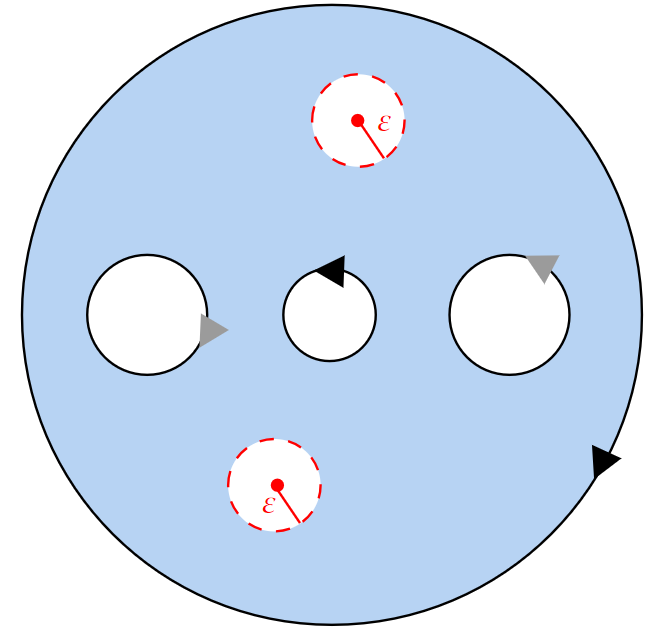
\includegraphics[width=14em]{Pics/1.png}
\caption{Fundametnal domain of Schottky uniformization in presence of punctures and conical points for $g=2$. The red circle indicate cutting a small circle of radius \textcolor{red}{$\delta$} from the fundamental domain, centerd at puncture or conical points. The blue region is the fundamental domain \textcolor{red}{$\singfund_{\delta}$}.}
\label{fig:1}
\end{figure}
\begin{figure}[h]
\centering
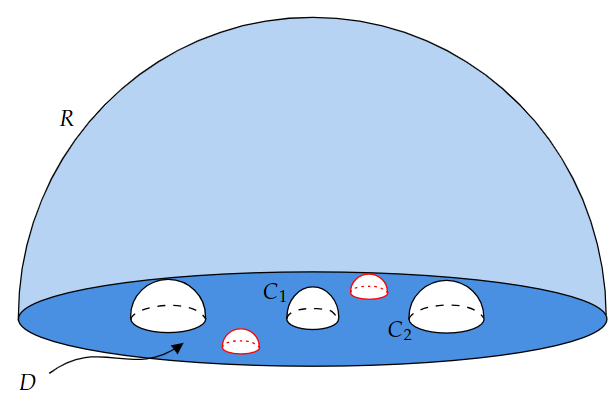
\includegraphics[width=18em]{Pics/2.png}
\caption{The three dimensional extension of fundamental domain \textcolor{red}{$\singfund_{\delta}$} in Figure \ref{fig:1}. \textcolor{red}{Correct the color for the fundamenal domain $\singfund_{\delta}$}.}
\label{fig:2}
\end{figure}

First, let's review the  homological construction in the absence of singularities. Consider a finitely generated purely loxodromic subgroup $\Sigma$ of $\PSLC$, namely a marked  Schottky group with a region of discontinuity $\Omega \subset\hat{\mathbb{C}}$ (see \cite{zograf1988uniformization,Taghavi2024classical} and Appendix.\ref{Schotkkyreview} for more details). The compact Riemann surface $X =\Omega\slash \Sigma$ is the conformal boundary of the corresponding hyperbolic three-manifold  $M = (\mathbb{U}^3\cup \Omega)\slash\Sigma$, where $\mathbb{U}^3 = \{(z,r) \; | \; z\in \mathbb{C}, r>0
\}$. Accordingly, the fundamental domain $\SchottkyFund$ can be extended to the upper-half space with a geodesic representative, as is shown in Figure \ref{fig:2} (forget the red hemispheres for now).

Set $\tilde\Omega=\mathbb{U}^3\cup \Omega $, and let $\compfontdi{S}=\compfontdi{S}(\mathbb{U}^3\cup \Omega)$ and $\compfontdi{B}=\compfontdi{B}(\mathbb{Z}\Sigma)$ denote the singular chain complex of $\mathbb{U}^3\cup \Omega$ and standard bar resolution complex for $\Sigma$, respectively. The key idea is to construct a 3-chain that represents $\mathbb{U}^3\cup \Omega$ in total complex $\text{Tot} \compfont{K}$ of the double homology complex $\compfontdii{K}= \compfontdi{S} \otimes_{\mathbb{Z}\Sigma} \compfontdi{B}$ as follows. Identify $R\subset \mathbb{U}^3$ (the blue region in Figure \ref{fig:2}) with $R\otimes[\;] \in \compfont{K}_{3,0}$ as the fundamental region of $\Sigma$ in $\mathbb{U}^3\cup\Omega$ such that $R\cap\Omega$ corresponds to the fundamental domain $\SchottkyFund$. Here $\partial''R=0$ and
\begin{equation}
\partial' R = -\SchottkyFund- \sum_{i=1}^{g} \big(H_i -L_i(H_i)\big) = -\SchottkyFund + \partial'' S,\label{pprimeR}
\end{equation}
where $H_i$ is a topological hemisphere and $S \in \compfont{K}_{2,1}$ is defined by
\begin{equation}
S = \sum_{i=1}^{g} H_i \otimes [L_i^{-1}].\label{}
\end{equation}
We can proceed similarly and obtain
\begin{equation}
\begin{aligned}
\partial'' S = -
\sum_{i=1}^{g} \big(H_i\otimes [\;] - L_i(H_i) \otimes [\;]\big),
\end{aligned}
\end{equation}
and
\begin{equation}
\begin{aligned}
\partial'S = L,\label{pprimeS}
\end{aligned}
\end{equation}
where $L= \sum_{i=1}^{g} C_i \otimes [L_i^{-1}] \in \compfont{K}_{1,1}$ and $C_i$ indicates Schottky circles shown in Figure \ref{fig:2}. Since the total complex $\text{Tot} \compfont{K}$ is equipped with the total differential $\partial= \partial'+(-1)^a \partial''$ on $\compfont{K}_{a,b}$, then the 3-chain $R-S \in (\text{Tot}\compfont{K})_3$ satisfies (see equations \eqref{pprimeR} and \eqref{pprimeS})
\begin{equation}
\partial (R-S) = -\SchottkyFund -L\overset{\text{def}}{=}-\Xi.\label{RmS}
\end{equation} 
As discussed in Section \ref{Renvolume}, it is important to note that defining the renormalized volume requires introducing a regularizing surface $f=\varepsilon$ near the conformal boundary. Consequently, the complex $R$ referenced earlier should be interpreted as $R\cap \{f\geq \varepsilon\}$. Additionally, as $r$ or $ \varepsilon$ approaches $0$, the cycle 
$\Xi$\footnote{It is straightforward to see that $\partial\hspace{.4mm}\Xi=0$ and if $\SchottkyFund$ and $\tilde{\SchottkyFund}$ are two choices of the fundamental domain for $\Sigma$ in $\Omega$, then $[\Xi]=[\tilde{\Xi}]$ for the corresponding classes in $H_2(\text{Tot}~\compfont{K})_2$.}  on $f=\varepsilon$
serves as an extension of the fundamental domain $\SchottkyFund$ (see \cite{aldrovandi_1997}), therefore $R-S$  is itself a consistent extension of $R$.

Adding punctures and conical points to the fundamental domain $\SchottkyFund$, amounts to cutting spheres around them, shown in Figure \ref{fig:2}. As demonstrated in Section \ref{Renvolume} (see also \cite{park2017potentials}), the regularizing surface $f=\varepsilon$   intersects the singularities, therefore to have it as a level-defining function we also need to remove the neighborhoods of each singularity at $(z_i,0)$ in $\mathbb{U}^3$.
\begin{figure}[h]
\centering
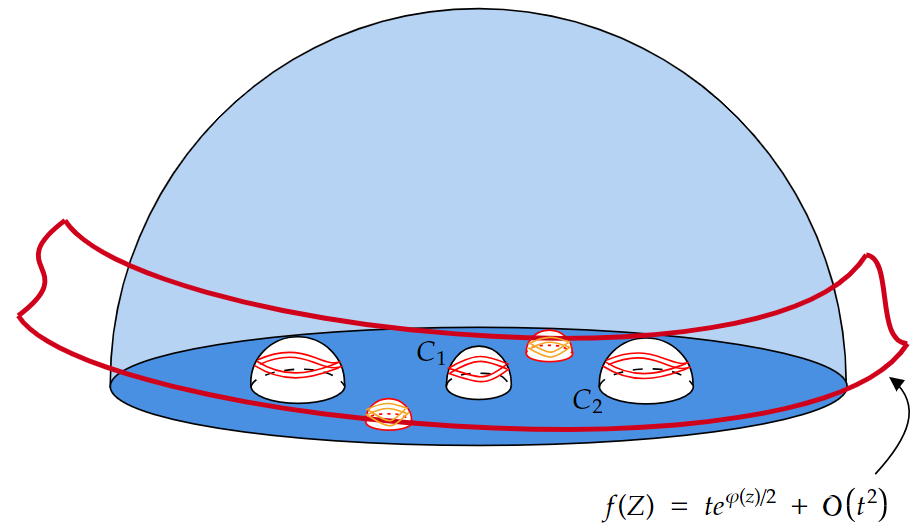
\includegraphics[width=23em]{Pics/3.png}
\caption{The regularizing surface $f(Z)$ which cuts through the fundamental region. \textcolor{red}{Substitute t with r. and order $r^3...$.}}
\label{fig:3}
\end{figure}
For $\varepsilon>0$, let
\begin{equation}
R_{\varepsilon} = R\cap\{f\geq\varepsilon\}\backslash \bigcup_{j=1}^{n}\big{\{}(z,r)\in\mathbb{U}^3\big| ~|(z,r)-(z_i,0)| \leq \tilde{\varepsilon}\big{\}},
\end{equation}
be the regularized truncated fundamental region. For $H_{i,\varepsilon}= H_i\cap R_{\varepsilon}$, the equation \eqref{pprimeR} changes to
\begin{equation}
\partial' R_\varepsilon = -\singfund_{\varepsilon}- \sum_{i=1}^{g} \big(H_{i,\varepsilon} -L_i(H_{i,\varepsilon})\big) = -\singfund_{\varepsilon} + \partial'' S_{\varepsilon},\label{pprimeReps}
\end{equation}
with 
\begin{equation}
S_\varepsilon = \sum_{i=1}^{g} H_{i,\varepsilon} \otimes [L_i^{-1}].
\end{equation}
Furthermore, again, 
\begin{equation}
\partial'S_\varepsilon  = \sum_{i=1}^{g} C_i \otimes [L_i^{-1}] = L,\label{pprimeSeps}
\end{equation}
and 
\begin{equation}
\partial' \singfund_{\varepsilon} 
=\partial'' L  + \sum_{j=1}^{n} c'_j\otimes [\;],\label{parD}
\end{equation}
where $c_j'$ is the trauncated circles around puncture and conical points shown in Figure \ref{fig:3}. Moreover, instead of \eqref{RmS}, by using equations \eqref{pprimeReps} and \eqref{pprimeSeps} one can see
\begin{equation}
\partial (R_{\varepsilon}-S_{\varepsilon}) = -\singfund_{\varepsilon}  -L\overset{\text{def}}{=}-\Xi_{\varepsilon}.\label{RmSeps}
\end{equation} 


\subsection{Cohomology in bulk: cohomology group and group cohomology}\label{CohomologyU3}
In this subsection, we construct double cohomology complex of $\mathbb{U}^3$ in presence of singularities (massive particles) within the context of Schottky uniformization. The cohomology construction starts with $\omega_3$:
\begin{equation}
\omega_3 = \frac{1}{r^3} ~\dd x\wedge \dd y\wedge \dd r= \frac{i}{2r^3}~\dd z\wedge \dd\bar{z}\wedge\dd r \in \compfont{C}^{3,0},
\end{equation}
the corresponding three-form on $\mathbb{U}^3$. It is an exact form since $\omega_3= \dd \omega_2$ with
\begin{equation}
\omega_2 = -\frac{i}{4r^2}~\dd z\wedge \dd\bar{z}\in \compfont{C}^{2,0}.\label{omega2}
\end{equation}
For the group element $\gamma = \begin{pmatrix}
a & b \\
c & d 
\end{pmatrix}\in \Sigma\subset \PSLC$, a straightforward calculations using the equation \eqref{deltatildew} yields
\begin{equation}
\begin{split}
\left(\delta\omega_2\right)_{\gamma^{-1}}&= \omega_2.\gamma-\omega_2 \\&
=\frac{i}{2} J_{\gamma}(Z)\Bigg(\left|c\right|^2 \dd z\wedge\dd\bar{z}-\frac{c\overline{(c z+d)}}{r}\dd z\wedge\dd r+\frac{\bar{c}(cz+d)}{r}\dd\bar{z}\wedge\dd r\Bigg),
\end{split}\label{deltaomega2}
\end{equation}
where $J_{\gamma}(Z)$ is defined in \eqref{Jgammaz}. It is important to note that in simplifying equation \eqref{deltaomega2}, we solely relied on the fact that $\text{det}(\gamma)=1$. Since 
\begin{equation}
\dd \delta\omega_2 =\delta \dd \omega_2 =\delta\omega_3,
\end{equation}
and $\omega_3$ is invariant under the  transformations by the group $\Sigma$, this implies that there exists $\omega_1\in \compfont{C}^{1,1}$ such that $\delta\omega_2=\dd\omega_1$. Specifically,
\begin{equation}
\begin{aligned}
\big(\omega_1\big)_{\gamma^{-1}} = -\frac{i}{8} \log \Big(
|r~c(\gamma)|^2 J_\gamma(Z)
\Big) \Big(
\frac{\gamma''}{\gamma'}dz -  \frac{\overline{\gamma''}}{\overline{\gamma'}}d\overline{z}
\Big),
\end{aligned}
\end{equation}
where $c(\gamma)$ is the left-hand lower element in the matrix representation of the generator $\gamma$. Proceeding further to compute  $\delta\omega_1\in \compfont{C}^{1,2}$, we find that (see  \cite{Takhtajan_2003})
\begin{equation}
\begin{split}
\left(\delta\omega_1\right)_{\gamma_1^{-1},\gamma_{2}^{-1}} &= -\frac{i}{8}\log\left(J_{\gamma}(Z)~\frac{\left|c(\gamma_2)\right|^2}{\left|c(\gamma_2\gamma_1)\right|^2}\right)\left(\frac{\gamma_2''}{\gamma_2'}\circ\gamma_1\gamma_1' \dd z -\frac{\overline{\gamma_2''}}{\overline{\gamma_2'}} \circ\gamma_1\overline{\gamma_1'} \dd \bar{z}\right)\\&-\frac{i}{8}\log\left(J_{\gamma_2}(\gamma_1 Z)~\frac{\left|c(\gamma_2\gamma_1)\right|^2}{\left|c(\gamma_1)\right|^2}\right)\left(\frac{\overline{\gamma_1''}}{\overline{\gamma_1'}}~\dd \bar{z}-\frac{\gamma_1''}{\gamma_1'}~\dd z\right).\label{deltaomega1}
\end{split}
\end{equation}
From the explicit calculations in equation \eqref{deltaomega1}, or simply by observing that
\begin{equation}
\dd \delta\omega_1 = \delta\dd\omega_1=\delta(\delta\omega_2)=0,
\end{equation}
we conclude that $\delta\omega_1$ is a closed. Therefore, there exists $\omega_0\in \compfont{C}^{0,2}$ such that $\delta\omega_1=\dd \omega_0$. \textcolor{red}{Additionally, using $H^{3}(\Sigma,\singrigon)$ , the antiderivative can be chosen such that $\delta\omega_0=0$.} Finally, since the total complex $\text{Tot} \compfont{C}$ is equipped with the total differential $D= \dd+(-1)^a \delta$ on $\compfont{C}^{a,b}$, then for \begin{equation}
\varpi= \omega_2-\omega_1-\omega_0\in (\text{Tot}\compfont{C})^2,\label{varpi}
\end{equation}
one gets
\begin{equation}
D\varpi = \omega_3.\label{Dvarpi}
\end{equation}
It is worth recalling that $\varpi$ represents an element of $H^{2}(X,\textcolor{red}{\singrigon})$, where $X$ can be the regularizing surface $f=\varepsilon$, which, as $r\rightarrow 0$ , becomes the conformal boundary of the manifold $M$.



\bibliographystyle{jhep.bst}
\bibliography{references}



\end{document}
